\documentclass{llncs}

\usepackage{ifpdf}
\ifpdf
  \usepackage[pdftex]{graphicx}
  \graphicspath{{./pdf/}{./jpeg/}{./eps/}}
  \DeclareGraphicsExtensions{.pdf,.jpeg,.png}
\else
  \usepackage[dvips]{graphicx}
  \graphicspath{{./eps/}}
  \DeclareGraphicsExtensions{.eps}
\fi

\usepackage[cmex10]{amsmath}
\usepackage{amsfonts}
\usepackage[noend]{algpseudocode}
\usepackage{algorithm}
\algnewcommand{\LineComment}[1]{\State \(\triangleright\) #1}
\usepackage[tight,footnotesize]{subfigure}
\begin{document}

\title{Bisection and Twisted Bidiagonal SVD on GPU for Big Matrices}

\author{Lu He\inst{1}, Yan Luo\inst{1}, Rui Liu\inst{1}, Hengyong Yu\inst{1}, Yu Cao\inst{1}, Xuzhou Chen\inst{3} and Seung Woo Son\inst{1}}

\institute{University of Massachusetts Lowell, Lowell MA 01854, USA
\and
Fitchburg State University, Fitchburg MA 01420, USA}

\maketitle
\begin{abstract}
Singular value decomposition (SVD) is one of the most important factorizations in matrix computation.
However, computing the singular values and their vectors is still time-consuming, especially when the dimension of matrices exceeds tens of thousands.
In this paper, we present a high performance approach called ``Bisection and Twisted'' (BT) for solving bidiagonal SVD. 
%Based on the bidiagonal SVD method and with a complexity of $O(n^2)$, the BT algorithm has three salient features:
%(1) it is shown to have weak data dependency, therefore can solve large SVD problems by splitting them into smaller ones; 
%(2) it can compute any subsets of singular values and corresponding vectors directly with computational complexity of $O(kn)$, making it suitable for applications that do not require the whole SVD calculation; and  
%(3) it needs only $O(kn)$ memory space for temporary variables, thus can work on memory-constrained platforms.
As modern general purpose GPUs have shown their extreme computational advantages in parallel computing, we implement the BT algorithm on single and multiple GPUs.
With our carefully designed GPU kernels, the BT algorithm is about $10$ times faster than MKL divide-and-conquer routine DBDSDC on 8-core 2.53GHz CPU, and $36$ times faster than CULA QR routine DBDSQR on the same GPUs.
Additionally,  the BT algorithm is able to compute SVD for matrices of size $1$ million by $1$ million with only two GPUs.
To the best of our knowledge, no implementation has achieved such a scale.

\end{abstract}

%\begin{IEEEkeywords}
%Singular Value Decomposition; Singular value; Singular vectors; GPU; Twisted factorizations; Bisection algorithm.

%\end{IEEEkeywords}

%\begin{abstract}
%The abstract should summarize the contents of the paper
%using at least 70 and at most 150 words. It will be set in 9-point
%font size and be inset 1.0 cm from the right and left margins.
%There will be two blank lines before and after the Abstract. \dots
%\end{abstract}
%

\vspace{-0.1in}
\section{Introduction} \label{sec:intro}
\vspace{-0.1in}
There is rapidly growing interest in singular value decomposition (SVD) in various fields,
including signal processing, computer vision, information retrieval, machine learning and information theory.
Yet, most algorithms for computing SVD are designed to solve problems with only small-scale data in acceptable time and space requirements due to their algorithmic complexities.
With the advent of the ``big data'' era, these algorithms are no longer adequate in terms of computational complexity and required memory space.

%A typical SVD algorithm can be broken down into two steps \cite{65SIAM}.
%The first step is to reduce the initial matrix to bidiagonal.
%The second step is to diagonalize the resulting matrix.
%Most of the literature focuses on the second step as algorithms in second step typically use iterative approaches \cite{58iter1,90iter2,65iter3} and thus take the bulk of the computation time depending on the accuracy requirement.

QR iteration is an algorithm that is widely used in sofeware application.
Jacobi algorithm is the one with the highest accuracy in practice \cite{97bookalgebra}.
However, the cost of $O(n^3)$ complexity with a big constant causes these algorithms very slow.
Divide-and-conquer (DC) is assumed to be the fastest algorithm for large matrices \cite{94DCSVD}.
It takes $O(n^{2.3})$ flops on average \cite{97bookalgebra}. 
But the major drawback of DC is the relatively low accuracy of the singular values when merging, let alone singular vectors. 
In summary, the prior works on SVD computations are either time-consuming or inaccurate.

In addition, all algorithms discussed above have three common disadvantages:
(1) heavy data dependence makes these SVD algorithms not suitable for parallelization and extension for other architectures;
(2) large memory space required for temporary variables dramatically limits the capability for computing singular values for very large matrices, and
(3) many application, such as principal component analysis (PCA), only require a small subset of the singular values and vectors, however, these algorithms are unable to calculate the subsets {\color{red}without the whole decomposition}.

In this paper, we present a new SVD approach called ``Bisection and Twisted'' (BT) algorithm and implement it on GPU. 
Compared to other algorithms, BT approach only requires $O(n^2)$ to complete SVD\cite{05UCB,09NLAAtwisted}.
Most importantly, there are three salient features that make BT algorithm attractive for very large matrices. 
First, the data dependency is weak in the BT algorithm, which make it an excellent candidate for parallel computing. 
Second, the algorithm can obtain a subset of $k$ singular values and its corresponding vectors in $O(kn)$ time. 
This is particularly useful for applications that do not require a complete SVD.
Third, the algorithm needs only $O(kn)$ memory space to store temporary variables, which is important for extending to large scale matrices in big data applications on memory constrained platforms.
We design a multi-GPU version of BT algorithm that can scale well with the matrix size. To the best of our knowledge, we are the first to achieve bidiagonal SVD on a 1 million by 1 million matrix using just two GPUs.
We also perform in-depth analysis on the GPU kernels for singular vector calculation, and present multiple optimization methods to further improve the SVD performance on GPUs.

The rest of the paper is organized as follows.
The Bisection and Twisted algorithm is given in Section \ref{sec:algorithm}.
Section \ref{sec:implementation} describes the implementation of the BT algorithm on GPUs, as well as the GPU specific optimizations.
Section \ref{sec:results} presents the experimental results and profiling analysis of GPU kernels.
Section \ref{sec:related} discusses the related work.
The conclusion and future work are in Section \ref{sec:conclusion}.



\vspace{-0.1in}
\section{Bisection and Twisted Algorithm} \label{sec:algorithm}
\vspace{-0.1in}
For an arbitrary matrix $A\in \mathbb{R}^{m \times n} (m>n)$, 
A SVD of an arbitrary matrix $A\in \mathbb{R}^{m \times n} (m>n)$ is the form $A = U \Sigma V^T$, where $U$ is a $m \times m$ orthogonal matrix, $V$ is a $n\times n$ orthogonal matrix, and $\Sigma$ is a $m\times n$ diagonal matrix.
A typical SVD algorithm can be broken down into two steps \cite{65SIAM}.
The first step is to reduce the initial matrix to bidiagonal by Householder transform.
The second step is to diagonalize the bidiagonal matrix.
Since Householder transform above has been optimized in paper \cite{LiuHouseholder}, we focus only on the second step that reduces a bidiagonal matrix to a diagonal matrix, for which the  ``bisection and twisted'' algorithm is designed.

%\begin{equation}
%A = Q B P^T
%\label{eq:householder}
%\end{equation}
%where $B \in \mathbb{R}^{m \times n}$ is a bidiagonal matrix of the form $ B = ( B_1, 0 )^T$.
%Here $B_1 \in \mathbb{R}^{n \times n}$ is a bidiagonal matrix. 
%Since $B^T B = (B_1^T, 0)(B_1, 0)^T = B_1^T B_1$,
%we assume, without loss of generality, that $B$ is a $n \times n$ bidiagonal matrix in this paper.
 
The bisection and twisted algorithm is divided into two phases:
(1) obtain the singular values of the bidiagonal matrix by bisection approach; and
(2) obtain the corresponding left and right singular vectors of every singular value by twisted factorization.
Next we illustrate these two phases in the following subsections.

\vspace{-0.1in}
\subsection{Bisection Algorithm}
\vspace{-0.1in}
Suppose $B$ is an upper bidiagonal $n \times n$ matrix with elements $b_{i,j}$ reduced by Householder transform \cite{10householder}.
The matrix $T = B^T B - \mu^2 I_n$ can be decomposed as
\begin{equation}
\label{eq:T}
T = B^T B - \mu^2 I_n = L D L^T ,
\end{equation}
where $\mu$ is a shift variable, $D=diag(d_1,d_2,\cdots,d_n)$ and $L$ is lower bidiagonal matrix, whose diagonal elements are $1$s and one-order subdiagonal are $l_{i}, (i=1,\cdots,n-1)$.
%are as below.
%\[ D =  \left( \begin{array}{cccc}
%d_{1} & 0     & \cdots & 0 \\
%0     & d_{2} & \cdots & 0 \\
%\vdots& \vdots& \ddots & \vdots \\
%    0 & 0     & \cdots & d_{n} \end{array} \right), \;\;\;\;
% L =  \left( \begin{array}{ccccc}
%     1&      &       &        &  \\
% l_{1}& 1    &       & 0      &  \\
%      & l_{2}& \ddots&        &  \\
%      & 0    & \ddots& \ddots &  \\
%      &      &       & l_{n-1}& 1
%\end{array} \right) \label{eq:l} \]
By substituting $L$ and $D$ into Eq. (\ref{eq:T}), we can get the following equations
\[ \left \{ \begin{aligned}
b_{1,1}^2 - \mu^2 &= d_1\\
b_{k-1,k-1} b_{k-1,k} &= d_{k-1} l_{k-1}\\
b_{k-1,k}^2 + b_{k,k}^2 - \mu^2 &= l_{k-1}^2 d_{k-1} + d_k
\end{aligned} \right . \label{eq:ldl} \]
where $k = 2,3,\cdots,n$.
Next, we define an auxiliary values $t_{k} = t_{k-1} * (b_{k-1,k}^2 / d_{k-1}) - \mu^2$, and then all the equations in Eq. (\ref{eq:ldl}) reduce to
\begin{equation}
\left \{
\begin{aligned}
d_1 = b_{1,1}^2 - \mu^2 \\
d_k = b_{k,k}^2 + t_{k}
\end{aligned}
\right .
\label{eq:negcount}
\end{equation}

Matrices $D$ and $T$ are two congruent symmetric matrices.
According to the Sylvester's law of inertia, both matrices $D$ and $T$ have the same numbers of positive, negative, and zero eigenvalues.
Thus, the number of negative elements in the diagonal of matrix $D$ is the number of singular values of matrix $T$.
We define a function denoted by $NegCount(\mu)$ to count the number of elements  in the diagonal of matrix $D$ that are negative. %described in Algorithm \ref{alg:negcount}.
%Algorithm \ref{alg:negcount} describes how $NegCount$ function works.
%Lines 3-7 calculate the negative number of singular values that are less than $\mu$.
%Since matrices $B$ and $B^T$ have the same singular values,
$NegCount(\mu)$ is also the number of the singular values of $B$ which are less than $\mu$.
%If the floating point arithmetic is monotonic, then $NegCount(x)$ is a monotonically non-decreasing function of $x$ \cite{95ETNAbisecion}.
% %\alglanguage{pseudocode}
\begin{algorithm}
%\small
\caption{NegCount in Bisection Algorithm}
\label{alg:negcount}
\begin{algorithmic}[1]
\Procedure{$\mathbf{NegCount}$}{$n, B, \mu$}
  \State $d=1$, $t=0$, $cnt=0$, $b_{0,1}=0$;
  \For {$k = 1 \to n$}
    \State $t = t * (b_{k-1,k}^2 / d) - \mu^2$;
    \State $d = b_{k,k}^2 + t$;
    \If {$d < 0$}
      \State $cnt++$;
    \EndIf
  \EndFor
  \State \Return $cnt$;
\EndProcedure
\end{algorithmic}
\end{algorithm}


%Algorithm \ref{alg:negcount} is used to count the number of singular values of matrix $B$ those are less than $\mu$.
%From the algorithm, the number of singular values in an arbitrary interval $[\mu_1,\mu_2)$ are $c_{\mu_2} - c_{\mu_1}$.
%Algorithm \ref{alg:bisection} is the bisection algorithm for calculating the singular values in interval $[l,u)$. Based on the definition of $NegCount$ the total number of singular values in $[l,u)$ is $n_u - n_l = NegCount(u) - NegCount(l)$.
%Lines 5-17 can be parallelized in bisection algorithm.
%In our implementation, we parallelize Line 5-17 of the bisection algorithm. 
%%\alglanguage{pseudocode}
\begin{algorithm}
%\small
\caption{Bisection Algorithm}
\label{alg:bisection}
\begin{algorithmic}[1]
\Procedure{$\mathbf{Bisection}$}{$val, n, B, l, u, n_l, n_u,\tau$}
  \If {$n_l \geq n_r$ or $l > u$}
    \State No singular values in $[l,u)$;
  \EndIf
  \State Enqueue ($l, u, n_l, n_u$) to Worklist;
  \While {Worklist is not empty}
    \State Dequeue ($a, b, n_a, n_b$) from Worklist;
    \If {$b - a < \tau$}
      \For {$i=n_a+1 \to n_b$}
        \State $val[i] = \min(\max((a+b)/2,a),b)$;
      \EndFor
    \Else
      \State $m = MidPoint(a,b)$;
      \State NegCount($n_m, B, m$);
      \State $n_m = \min(\max(n_m,n_a),n_b)$;
      \If {$n_m > m_a$}
        \State Enqueue ($a, m, n_a, n_m$) to Worklist;
      \EndIf
      \If {$n_m < m_b$}
        \State Enqueue ($m, b, n_m, n_b$) to Worklist;
      \EndIf
    \EndIf
  \EndWhile
\EndProcedure
\end{algorithmic}
\end{algorithm}


%\subsubsection{Weak Data Dependency of Bisection Algorithm}
%~
%The efficiency of our algorithm is based on the assumption that the data dependencies for both separating and calculating phases are weak so that we could divide the big problem into smaller but loosely coupled components. Since the singular values are all positive, we assume that the boundary containing all the singular values is $[0, ug)$, where the upper bound $ug$ can be calculated by Gershgorin circle theorem\cite{gershgorin}.
%
%After obtaining the boundary, we divide the interval $[0,ug)$ into $p$ subintervals, and each subinterval $[l_i,u_i)$ can be calculated as follows:
%\begin{eqnarray}
%l_i &=& (ug/p) * (i-1)\\
%u_i &=& (ug/p) * i ,
%\end{eqnarray}
%where $i = 1, 2, \cdots, p$. Then we can calculate the numbers of singular values $n_{l_i}$ and $n_{u_i}$ that are less than $l_i$ and $u_i$ as follows, respectively:
%\begin{eqnarray}
% n_{l_i} = NegCount(l_i) \\
% n_{u_i} = NegCount(u_i) .
%\end{eqnarray}
%$n_{u_i} - n_{l_i}$ is the number of singular values in interval $[l_i,u_i)$ and $n_l, n_l+1, ..., n_u-1$ are the indices of these singular values. 
%The interval can be divided 
%We thus illustrate that the data dependence is weak when dividing the interval
%to subintervals.
%
%Now, we show that the data dependency in bisection algorithm is also weak in the calculation phase (Algorithm \ref{alg:bisection}).
%Suppose $[l,u)$ is an subinterval containing several singular values of a matrix.
%$n_l$ and $n_u$ are the numbers of singular values that are less than $l$ and $u$, respectively.
%How is the bisection algorithm able to calculate an arbitrary singular value $v$ with index $(n_l+k)$ in an subinterval $[l,u)$?
%After several bisection iterations, the subinterval $[l,u)$ reduces to $[v_1,v_1+\tau)$, whose $NegCount$ are $(n_l+k-1)$ and $(n_l+k)$, respectively.
%Since $v$ is in the subinterval $[v_1,v_1+\tau)$, we know that $| v_1 - v | < \tau$, and if $\tau$ is small enough, we stop the iteration and take $v_1$ as calculated singular value with index $(n_l+k)$.
%The whole procedure of bisection algorithm requires only $NegCount$ function without the information of other singular values.
%
%\subsubsection{Error Analysis}
%~
%
%In theory, the bisection algorithm is bound to the upper limit of error between actual value and calculating value, which can be set according to particular applications. 
%The selection of an error tolerance $\tau$ greatly impacts the execution time of the algorithm. 
%Large error tolerance will allow us to solve the problem quick but result in low accuracy.
%On the other hand, too small value for $\tau$ may fail to reach the required accuracy.
%Based on our tests, we can obtain the singular values with error tolerance less than $10^{-16}$.

\vspace{-0.1in}
\subsection{Twisted Algorithm}
\vspace{-0.1in}
%The second phase of our algorithm, twisted algorithm, calculates the corresponding singular vectors.
%It has advantages over existing approaches such as the power method\cite{08power}, which can only find the largest singular value and the corresponding singular vector, and inverse iteration\cite{11iterative}, which does not guarantee the accuracy and orthognality of the singular vectors when the singular values are clustered. In contrast, the twisted algorithm can calculate  orthogonal singular vectors with adequate accuracy \cite{09NLAAtwisted}. 

Suppose $\lambda$ is a singular value of bidiagonal matrix $B \in R^{n \times n}$.
Then the matrix $B^T B - \lambda^2 I$ can be decomposed as
\begin{equation}
B^T B - \lambda^2 I_n = L D_L L^T = U D_U U^T ,
\end{equation}
where $D_L=diag(\alpha_1, \cdots, \alpha_n)$, $D_U = diag(\beta_1, \cdots, \beta_n)$, 
$L$ is lower bidiagonal matrix, whose diagonal elements are $1$s and one-order subdiagonal are $l_{i}, (i=1,\cdots,n-1)$, 
$U$ is upper bidiagonal matrix, whose diagonal elements are $1$s and one-order superdiagonal are $u_{i}, (i=1,\cdots,n-1)$. 
%\[ L =  \left( \begin{array}{ccccc}
%     1&      &       &        &  \\
% l_{1}& 1    &       & 0      &  \\
%      & l_{2}& \ddots&        &  \\
%      & 0    & \ddots& \ddots &  \\
%      &      &       & l_{n-1}& 1
%\end{array} \right), \;\;\;\;
% U =  \left( \begin{array}{ccccc}
%  1 & u_{1}&       &       &  \\
%    & 1    & u_{2} & 0     &  \\
%    &      & 1     & \ddots&  \\
%    & 0    &       & \ddots& u_{n-1} \\
%    &      &       &       & 1
% \end{array} \right) \]
%$L$ is left bidiagonal matrix, $U$ is upper bidiagonal matrix.
%The diagonal elements in $L$ and $U$ are 1s.
%The subdiagonal elements are $l_k$ in $L$, and the superdiagonal elements are $u_k$ in $U$, separately.

Given the $LDL^T$ and $UDU^T$ decomposition, the twisted factorization of the shifted matrix is shown as
\begin{equation}
B^T B - \lambda^2 I = N_k D_k N_k^T ,
\label{eq:twisted}
\end{equation}
where $k = \arg \min \gamma$, and $\gamma$ is defined as
$\gamma = (\beta_1, \beta_2 - \alpha_2 * l_1, \cdots, \beta_i - \alpha_i * l_{i-1}, \cdots, \beta_i - \alpha_i * l_{i-1}, \alpha)$, 
%in Eq. (\ref{eq:gamma}).
%\begin{equation}
%\label{eq:gamma}
%k = \arg \min_{1\le i \le n} \gamma_{i} =
%\begin{cases}
%\beta_1 & \text{if } i=1 \\
%\beta_i - \alpha_i * l_{i-1} & \text{if } 2\le i\le n-1\\
%\alpha_n & \text{if } i=n
%\end{cases}
%\end{equation}
$D_k$ is diagonal matrix, $N_k$ is a twisted combination of the partial lower triangular $L$ and the partial upper triangular $U$.
%\begin{equation}
%N_k =  \left( \begin{array}{cccccccc}
% 1& & & & & & & \\
% l_{1}& \ddots& & & & 0& & \\
% & \ddots& 1& & & & &  \\
% & & l_{k-2}& 1 & & & & \\
% & & & \eta_k& 1& u_k& & \\
% & & & & & 1& \ddots& \\
% & & 0& & & & \ddots& u_{n-1}\\
% & & & & & & & 1 \end{array} \right)
%\end{equation}
%\begin{equation}
%\eta_k = \begin{cases}
%0 & \text{if } i=1 \\
%\frac{l_{k-1}\alpha_{k-1}}{(\alpha_{k-1} - v_{k-1}^2 \beta_{k+1})} & \text{if } 2\le i\le n-1\\
%\l_{n-1} & \text{if } i=n
%\end{cases}
%\end{equation}

Thus, the corresponding singular vector of $\lambda$ can be obtained by solving the following matrix equations and then normalizing the solution:
\begin{equation}
\label{eq:unnorm}
N_k^T Z_k = I_k ,
\end{equation}
 where each column in matrix $Z_k$ is the non-normalization solution of singular vector corresponding to $\lambda$, and $I_k$ is a unitary matrix.

%One advantage of BT algorithm is that it can be applied to cases where singular values are clustered together.
%\textcolor{red}{
Suppose $m$ is the multiplicity of singular values of matrix $B$. 
The algorithm selects the indices of the first $m$ minimum values of $\gamma$. %(May need some more clarification????)} 
Each index $k$ in $m$ has a different twisted factorization, and thus the singular vector can be obtained by solving its own Eq. (\ref{eq:unnorm}). These singular vectors are also orthogonal to each others\cite{09NLAAtwisted}.
%%\alglanguage{pseudocode}
\begin{algorithm}
%\small
\caption{Twisted Factorization}
\label{alg:twisted}
\begin{algorithmic}[1]
\Procedure{$\mathbf{Twisted}$}{$q, n, B, \mu$}
  \LineComment $l$ is the number of different singular values, $l\le n$;
  \For {$i = 1 \to l$}
    \State Computes matrix $S = B - \mu_i^2 I$;
    \State Computes $LDL'$ decomposition $S = LD_LL'$;
    \State Computes $UDU'$ decomposition $S = UD_UU'$;
    \State Computes $\gamma$ based on Eq \ref{eq:gamma};
    \State Find the number $m$ of clustered singular values $\mu$;
    \State Find $m$-th minimum $k = min_j  |\gamma(j)|$;
    \For {each k}
    \State $z_k = 1$, $z_{k-1} = -L_{k-1,k}$, $z_{k+1} = -U_{k,k+1}$;
    \For {$j = k+2 \to n$}
      \State $z_j = -U_{j-1,j}*z_{j-1}$
    \EndFor
    \For {$j = k-2 \to 1$}
      \State $z_j = -L_{j+1,j}*z_{j+1}$
    \EndFor
    \State Scale vector $q = z/||z||_2$;
    \EndFor
  \EndFor
\EndProcedure
\end{algorithmic}
\end{algorithm}

%Algorithm \ref{alg:twisted} is the algorithm to obtain the corresponding singular vectors of given singular values.
%Lines 4-7 are two obtain the parameter $\gamma$.
%Obtain the multiplicity of a singular value and their corresponding minimum values are described in Lines 8-9.
%Lines 10-16 are to calculate the singular vectors and normalize them.
%%We completely parallelize the twisted factorization to speed up the algorithm on GPU architecture.
%The cost for every singular vector transformation is $O(n)$, and the total cost of the transformations is $O(n^2)$.



\vspace{-0.1in}
\section{Implementation and Optimization on GPU} \label{sec:implementation}
\vspace{-0.1in}
\subsection{Singular Value Kernels} \label{sec_svalue}
\vspace{-0.1in}
To obtain the singular values, we divide the whole interval containing all the singular values into several subintervals, which can be computed in parallel. 
The whole interval can be calculated with Gershgorin circle theorem \cite{gershgorin}.
Each subinterval can then be assigned to one GPU block {\color{red}(which consists of threads and is executed by a multiprocessing unit concurrently)} for calculation.
Because there is a limit on the maximum number of threads for each GPU block,
the number of singular values in a subinterval must not exceed that maximum number. Otherwise, the computation will have to be wrapped into two or more sequential phases to complete.
Therefore how to divide the interval is critical for the performance of
computing singular values. We consider two different partition
strategies as described below. 
\begin{figure}[hbpt]
\vspace{-0.3in}
\centering
  \subfigure[Equal Length Division]
  {
  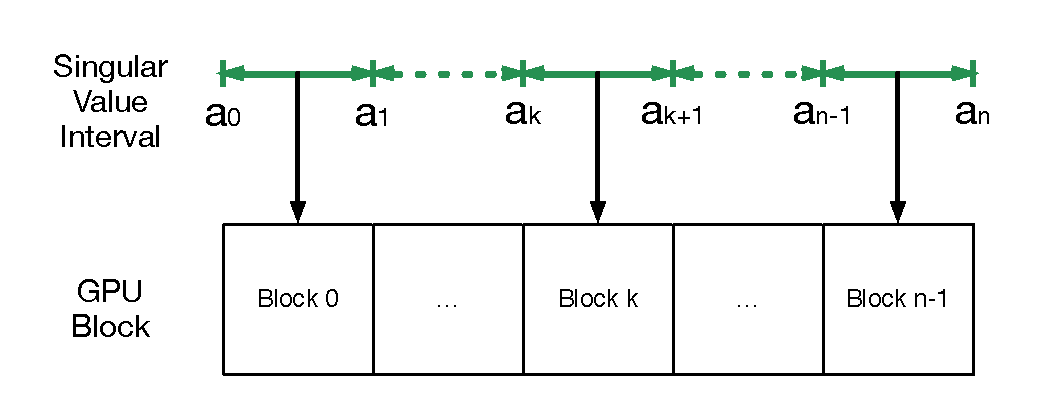
\includegraphics[width=0.45\textwidth]{length_interval}
  \label{fig:length_interval}
  }
  \subfigure[Equal Number Division]
  {
  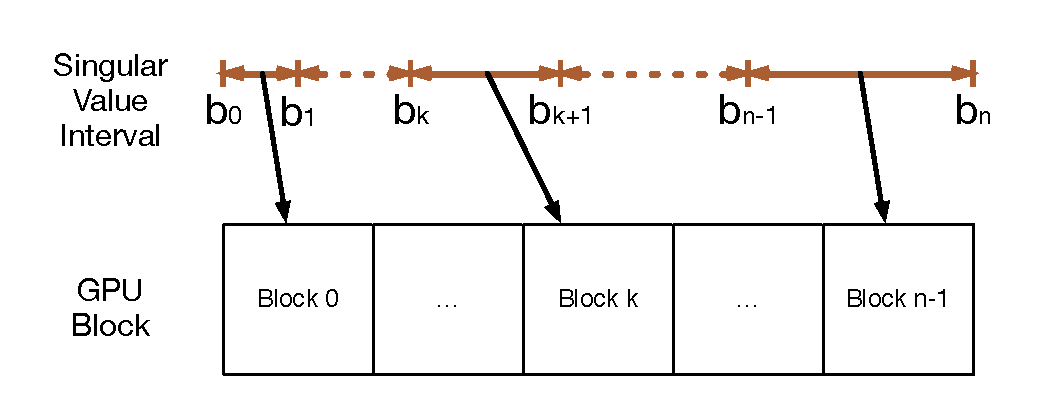
\includegraphics[width=0.45\textwidth]{number_interval}
  \label{fig:number_interval}
  }
\vspace{-0.1in}
  \caption{Division Strategies for Partitioning Interval  $[a_0, a_n)$.}
\vspace{-0.3in}
\end{figure}

The first (na\"{\i}ve) strategy is to divide the interval into chunks of equal length as shown in Fig.\ref{fig:length_interval}.
The whole interval $[a_0, a_n)$ is divided into $n$ subintervals with
the same length (i.e. same number of matrix elements). However, each
such subinterval might not contain the same number of singular values.
Mathematically, this strategy can be expressed as
$a_{k+1}-a_k = a_{k}-a_{k-1}$. However, $NegCount(b_{k+1})-NegCount(b_{k}) = NegCount(b_{k})-NegCount(b_{k-1})$ is not necessarily true. We call this strategy as {\it equal length division}.

Such ``equal length division'' strategy has issues in load balancing on 
parallel computing resources, as the number of singular values in each
subinterval is not uniform. As a result,
the SVD workload cannot be easily balanced on GPU's processing cores to achieve a satisfactory speedup because the optimal number of subintervals is dependent on multiple factors, such as the maximum number of threads, the number of threads in a GPU warp, and the size of matrix.
The maximum number of threads per block determines the minimum number
of subintervals that are assigned to corresponding GPU blocks.
In addition, the number of threads in a GPU warp assigned to a subinterval affects the GPU utilization level.

We have conducted experiments to understand the trade-offs between subinterval length and the GPU execution efficiency. 
Smaller subintervals will lead to a larger number of subintervals, which cause the GPU warp execution to be less efficient. 
For example, our experiments show that if $512$ subintervals are used, the efficiency of GPU warp execution ranges from only 12.38\% to 52.15\% when the matrix size increases from $1,000$ to $17,000$.
That is, only half of the threads in a warp work in parallel at most. This is because  (1)
 there are fewer singular values than the number of warps, leading the cores under-utilized; and 
(2) the warps are stalled due to memory accesses.
{\color{red}When the subinterval becomes larger, some block may get more singular values than its capability.}
In order to achieve a higher speedup, we could try to find the optimal number of subintervals, or the number of blocks, based on experimental results. 
However, because of the uneven number of singular values within subintervals, the speedup for equal length division remains very limited, which motivates us to search for a better partition method.

Our novel strategy is to divide the whole interval by the number of singular values, as shown in Fig.\ref{fig:number_interval}. We call this approach {\it equal number division}. 
Specifically, we divide the interval $[b_0,b_n)$ into $n$ subintervals, each of which has the same number of singular values. 
However, the length of a subinterval is not necessarily equal to others.
The mathematical representation can be written as $NegCount(b_{k+1})-NegCount(b_{k})=NegCount(b_{k})-NegCount(b_{k-1})$ but $b_{k+1}-b_k = b_{k}-b_{k-1}$ does not necessarily hold anymore.
This equal number division significantly improves the load balancing on GPU cores, helping achieve a better speedup, as we show the performace evaluation in Figure \ref{fig:compare_value_kernel}.

%The convergence of bisection algorithm on a splitting point makes it possible to compute the number of singular values before actually computing
%the values themselves. The splitting point can be easily found by applying several $NegCount$ functions on the interval. Specifically, we design a method to find the boundary points of such subintervals, as shown in Algorithm \ref{alg:numsub}.
%Line 2 is to obtain the whole interval of matrix $B$.
%Lines 4-5 find the midpoint of interval and its corresponding $NegCount$.
%Lines 6-15 make use of loop to find the split point of number division by bisection algorithm.
%Line 6-16 make use of loop to find the split point of number division by bisection algorithm.
%\begin{algorithm}
%\small
\caption{Equal Number of Singular Value Subinterval Algorithm}
\label{alg:numsub}
\begin{algorithmic}[1]
\Procedure{$\mathbf{Number\_Divide}$}{$n, B, t, \tau$}
  \State Obtain singular value boundary $[l,u)$ of matrix $B$;
  \State Define the thread ID $i$, $i<t$;
  \Comment t is total threads
  \State $mid = inside(l, u, B)$;
  \State $n_m = NegCount(n, B, mid)$;
  \While {$n_m \ne (i+1)n/t$ and $mid-l > \tau$}
    \If {$n_m \ge (i+1)n/t$}
      \State $u=mid$;
      \State $n_u=n_m$;
    \Else
      \State $l=mid$;
      \State $n_l=n_m$;
    \EndIf
    \State $mid = inside(l, u, B)$;
    \State $n_m = NegCount(n, B, mid)$;
  \EndWhile
  \State save the division point $mid$ and $n_m$.
\EndProcedure
\end{algorithmic}
\end{algorithm}


The significant advantage for the equal number division strategy is that, more singular values can be calculated with the equal number division strategy than equal length division strategy.
Our experiment results show that equal number division outperforms length division strategy:
The warp execution efficiency in equal number division version can reach 92.97\%-96.13\%.

\vspace{-0.15in}
\subsection{Singular Vector Kernel} \label{sec_svector}
\vspace{-0.1in}
Since the singular vectors are two $n\times n$ dense matrices, as the matrix size increases, there is increasing pressure on memory storage because the size of the fast shared memory is limited in GPU architectures.
It is impracticable to move all the matrix entries to the shared memory when matrix size becomes extremely large.

Based on the twisted algorithm, the required memory size $M$ on GPU is determined by matrix size $n$ and the size of floating number $S$ in equation $M = 5 * S * n^2$.
For example, the maximum matrix size with $4$-bytes floating number values is about $10000$ for a GPU with $2$GB GPU memory. 
For matrices larger than that, we need to explore multiple GPUs to scale its performance as described in Section \ref{sec_mgpu}.

We initially implement the twisted algorithm with row-major matrix stored in the global memory
of a GPU system. 
We observe the heavy usage of global memory, which is
the slowest memory component on GPUs. 
Further analysis reveals that about 50\% of global memory transfers are read-after-write. Since it is a waste of time to read from global memory after writing to global memory,
we could improve the memory access performance by copying these values into the local memory and shared memory of the GPU.
The way to store matrix elements (column major or row major) is also critical as the memory accesses could be coalesced if the matrix elements
can be read and computed in large chunks. We present the results
of such optimizations in Section \ref{sec:results}.

% as we depict
%the baseline global load/store transactions in Figure \ref{fig:transaction} (the leftmost bars).
%\begin{figure}[hbpt]
%\centering
%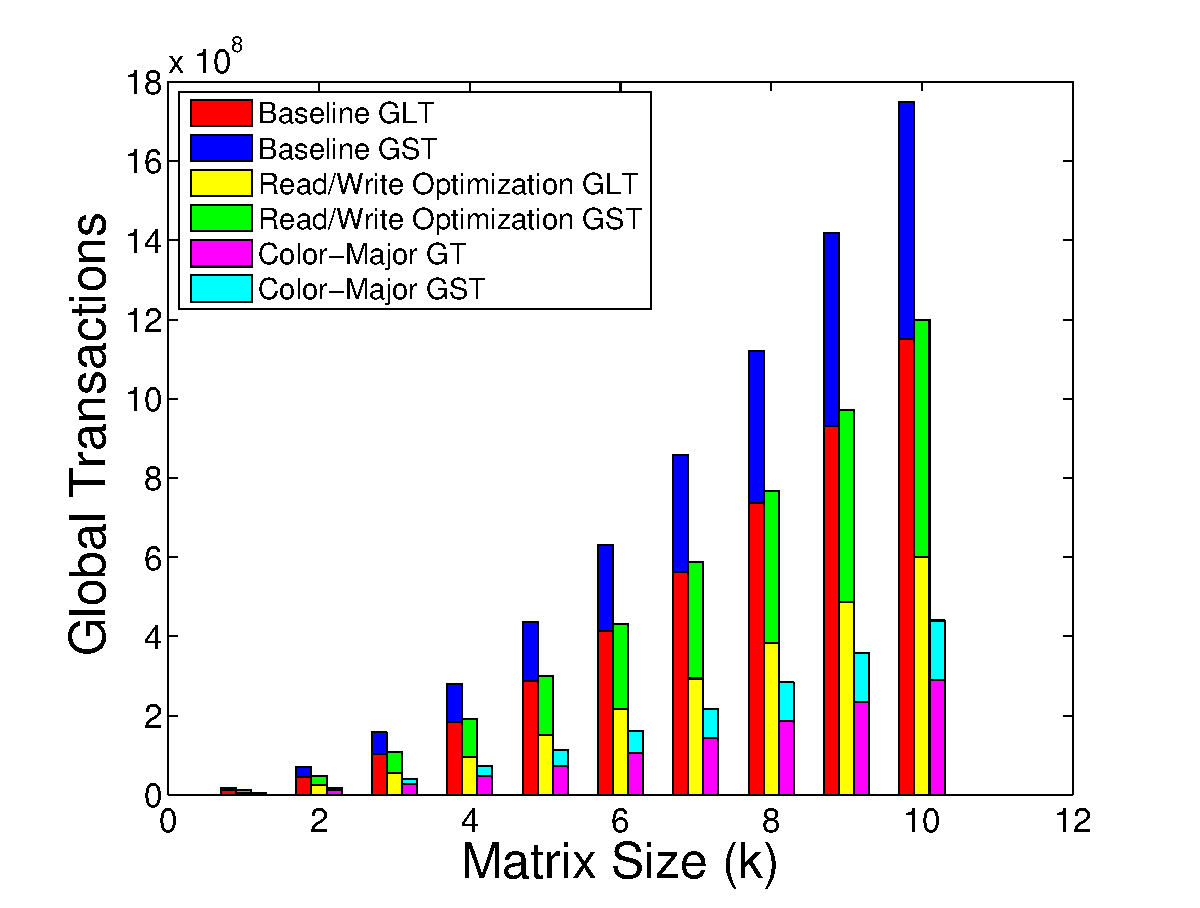
\includegraphics[width=0.5\textwidth]{transaction}
%\caption{Transactions on Singular Vector Design. \textcolor{blue}{GLT represents Global Load Transaction. GST presents Global Store Transaction}}
%\label{fig:transaction}
%\end{figure}
%%\begin{figure}[hbpt]
%%\centering
%%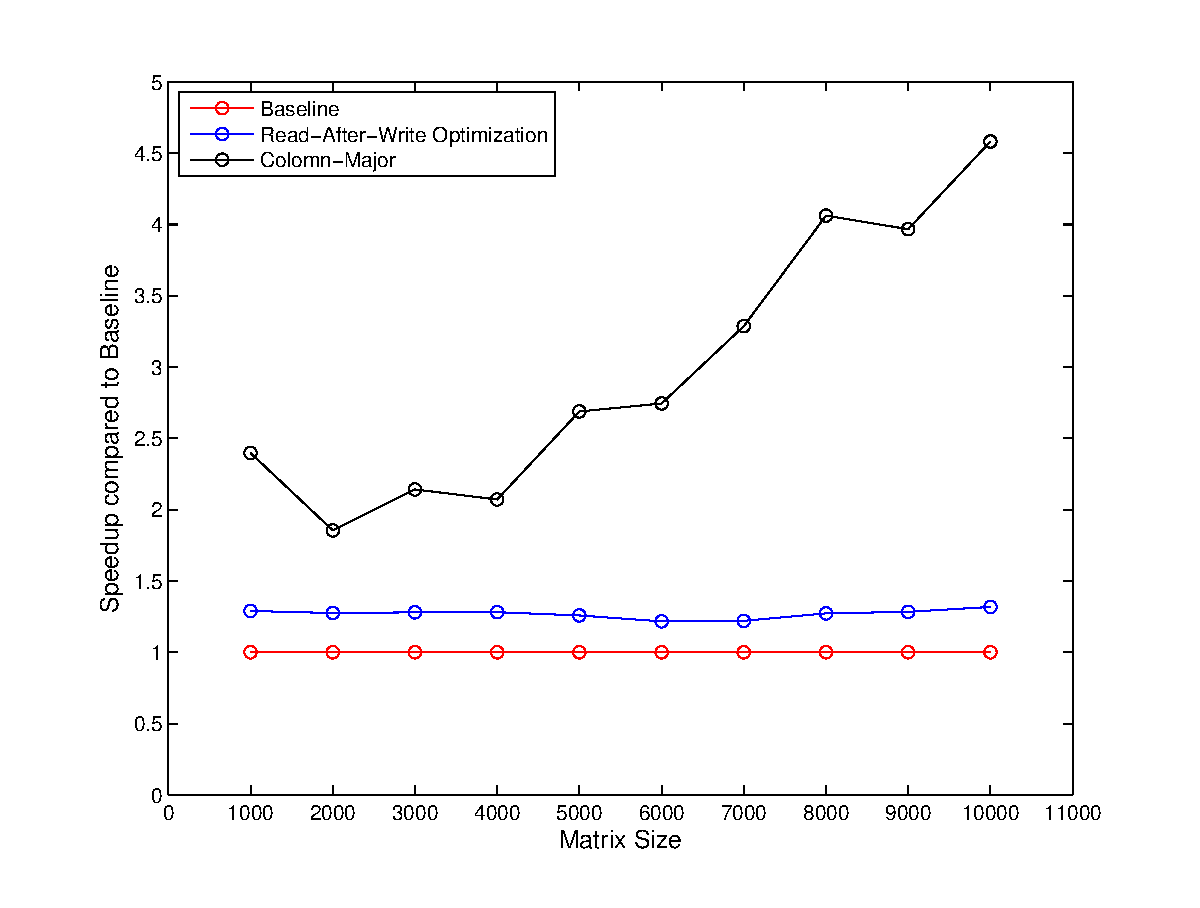
\includegraphics[width=0.5\textwidth]{vector_kernels}
%%\caption{Transactions on Singular Vector Design}
%%\label{fig:vector_kernels}
%%\end{figure}
%Read transactions are about twice of the write transactions on the global memory.
%Further analysis reveals that about 50\% of global memory transfers are read-after-write.
%Since it is a waste of time to read from global memory after writing to global memory,
%we improve the memory access performance by copying these values into the local memory and shared memory of the GPU.
%The global read transactions are reduced by 50\% compared to the baseline, while the write transactions remain the same, as shown as ``read/write optimization'' in Figure \ref{fig:transaction}. The speedup reaches to 1.2X compared to the baseline.
%To further optimize the access to the global memory,
%we change the matrix arrangement from row-major to column-major in the global memory. 
%As a result, the global load/store transactions are reduced by 50\%/25\% compared to ``read/write optimization'', respectively. 
%This is because column-major matrix have coalesced global memory accesses, which saves hundreds of transactions per thread. The speedup rises up to 4.5X compared to the baseline.

\vspace{-0.15in}
\subsection{Solution to Big Matrices} \label{sec_huge}
\vspace{-0.1in}
In our design, the maximum number of singular values can be processed on a singular GPU is $m_b = subinterval\_size \times thread\_block\_size$,
while the maximum number of singular vectors are determined by $m_t = \sqrt{U / (5 * S)}$,
where $U$ is the memory size of GPU, $5$ is the number of arrays required for a pair of singular vectors.
Usually, $m_b$ is much larger than $m_t$.
For Tesla K40c with 16GB memory, $m_t = 24K$, while $m_b = 262K$.
However, when the matrix size is larger than $m_t$, even larger than $m_b$,
the GPU kernels cannot obtain all singular values and vectors any more with a single GPU.
Therefore we derive a divide-and-conquer architecture to solve the huge matrix size as explained in this section.

When the size of a matrix is less than $m_b$ but larger than $m_t$,
we only need to divide the singular vectors into small sets, each of which can be processed by a single GPU.
However, if the matrix size is larger than $m_b$, we should divide both singular values and singular vectors into smaller partitions.
The singular value computations can be partitioned using $m_b$ directly, i.e., there are $l_b = \lfloor(n/m_b)\rfloor + 1$ partitions, each of which has $\lfloor(n/l_b)\rfloor$ singular values.

The division of singular vectors should take memory size into consideration.
The maximum number of partitions $l_t$ can be derived from Equation $l_t = \sqrt{U/(5 * n * 4)}$, 
where $n$ is matrix size.
Thus, there should be $\lfloor(n/l_t)\rfloor+1$ partitions with
$\lfloor(n/l_t)\rfloor$ singular vectors in each partition.

\vspace{-0.15in}
\subsection{Multiple GPUs on a server}\label{sec_mgpu}
\vspace{-0.1in}
We implement the multiple-GPU version with Pthread libraries on one server
to control data partition and assignment to GPUs.
Pthread is a nature choice for controlling multiple GPUs on a single server
because it uses shared memory architecture, dramatically reducing overheads
on data sharing. We also design an extensible interface between CPU and GPU,
 which is easy to scale to physical distributed GPUs, compared to CUDA asynchronization interface. In our design, each thread takes control of one GPU.

When matrix size becomes huge, the load balancing among multiple GPUs will be a problem for performance as shown in column 2 of Table \ref{tab:hugeResultTesla}.
To conquer this issue we also introduce a dynamic load-balancing method for a better speedup, where a GPU will take new tasks on unfinished subintervals as soon as it finishes its prior task.



\section{Experimental Results}
\label{sec:results}
In this section, we evaluate the performance of our bisection and twisted algorithm and compare it with prior SVD implementations on CPUs and GPUs.
We also evaluate the performance of BT on huge matrices of size more than $100K$. 
To our knowledge, this has not been done in any of the prior work so far. 
%In addition, we discuss the GPU kernel profiling results to show how to further optimize our implementations. 

We implement the proposed BT algorithm on three different GPUs: GeForce 750 Ti, Quadro 600 and Tesla K40c,
which differ in architecture, memory size and bandwidth.
Their specifications are listed in Table \ref{tab:spec}. 
In our implementations, we set the number of threads per GPU block as 512, which brings the better performance than other possible block sizes.
For the multi-GPU version of BT, we use a mixture of these GPUs that reside in the same server to scale up the size of matrices. 
%It is worth noting that our multi-GPU version of BT algorithm can be extended to physically distributed GPUs, i.e., GPUs on different hosts connected via a high speed network. 
%This part is however beyond the scope of this paper. 
\begin{table}[h]
\vspace{-0.2in}
\caption{Specifications of Different GPUs}
\vspace{-0.1in}
\centering
\begin{tabular}{|c|c|c|c|}
\hline
Specifications & GeForce 750 & Quandro 600 & Tesla K40 \\ \hline
Architecture   &     Maxwell &       Fermi &    Kepler \\ \hline
CUDA Cores     &         640 &          96 &      2880 \\ \hline
TFLOPS         &       1.306 &       0.246 &      4.29 \\ \hline
GPU Clock      &    1268 MHz &    1280 MHz &   745 MHz \\ \hline
Mem Size       &        2 GB &        1 GB &     12 GB \\ \hline
Mem Bandwidth  &   86.4 GB/s &   25.6 GB/s &  288 GB/s \\ \hline
\end{tabular}
\label{tab:spec}
\vspace{-0.5in}
\end{table}

\subsection{Comparison to Existing SVD Implementations}
We generate random bidiagonal matrices with double precision numbers in the range between 0 and 1.
In order to achieve high confidence on the results, we generate 10 random matrices, and for each matrix, our SVD algorithm is executed 10 times on a GPU (or two GPUs).
%The average performance does not vary much when more matrices and more times are used.
The standard deviation of their execution time is very small, so we report the average execution time across the 100 runs as the performance results.

We compare our algorithm with CULA GPU library \cite{cula}, Intel MKL library \cite{mkl}, Sheetal's QR implementation on S1070 \cite{09IPDPSQR}, and Liu's DC implementation on M2070 \cite{13CFDC}.
We measure the performance of CULA on Tesla K40c, and that of Intel MKL on an 8-core 2.53GHz CPU.
Until now, CULA library only has a QR based routine called culaDbdsqr.
Intel MKL library has both DC routine DBDSDC and QR routine DBDSQR. We select a faster routine DBDSDC for a comparison.
For Sheetal's \cite{09IPDPSQR} and Liu's \cite{13CFDC} implementation, we use the experimental results presendted in their paper. 

\begin{figure}[hbpt]
\vspace{-0.3in}
\centering
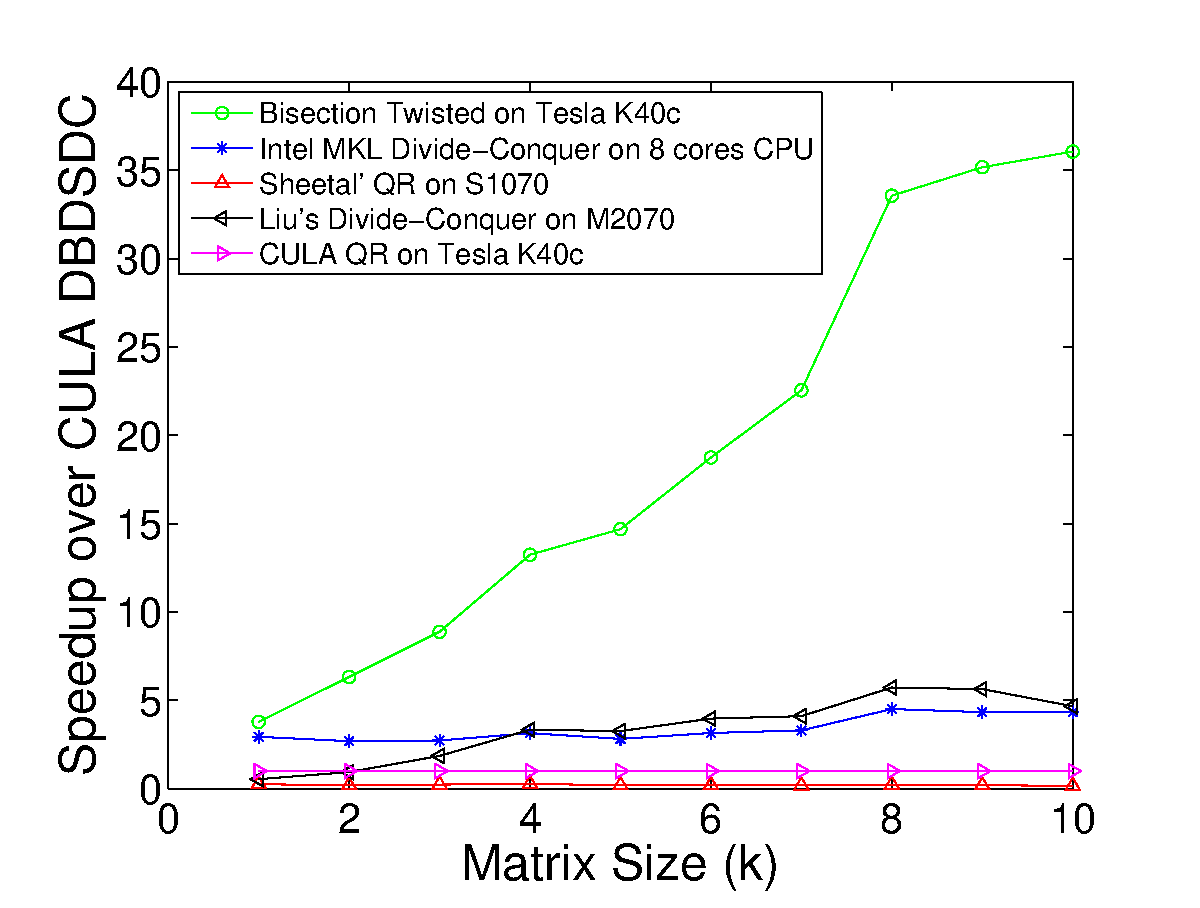
\includegraphics[width=0.5\textwidth]{svd_speedup}
\vspace{-0.2in}
\caption{Overall Performance Comparison}
\label{fig:svd_speedup}
\vspace{-0.3in}
\end{figure}
Figure \ref{fig:svd_speedup} shows the performance comparison of BT
implementation on Tesla K40c GPU to other existing libraries
and implementations.
The x-axis is the size of input matrix, and the y-axis is the speedup
using CULA QR routine DBDSQR as the baseline.
Our BT algorithm achieves a speedup of 3.8 to 36 over CULA culaDbdsqr routine,
while Intel MKL DBDSDC routine has a 2.9 to 4.3 speedup on a 8 core CPU and Liu's implementation achieves only 0.5 to 4.7 speedup over CULA library.
On the other hand, Sheetal's implementation is about 3 to 5.3 times slower than CULA library.

The performance of BT scales well when the matrix size becomes large.
Overall, we achieve a speedup of 1.3 to 8.3 over the Intel MKL
DC implementation on CPU, 4 to 7.2 over the Liu's
DC method on GPU, and 15 to 288 over the QR implementation in the work by Sheetal et al.
Now let us take a look at each of the algorithms from the perspective of matrix size, Sheetal's QR implementation and Liu's DC implementation do not work at all when the dimensions of matrices are larger than 14K by 14K on their GPU with memory size of 16GB and 6GB, respectively. In contrast, in our implementation, the matrix size could reach 1 million by 1 million as shown in Table \ref{tab:hugeResultTesla}.

\subsection{Performance Comparison on Different GPUs}

\subsubsection{Singular Value Computation}
\begin{figure}[hbpt]
\vspace{-0.3in}
\centering
  \subfigure[Execution time]
  {
    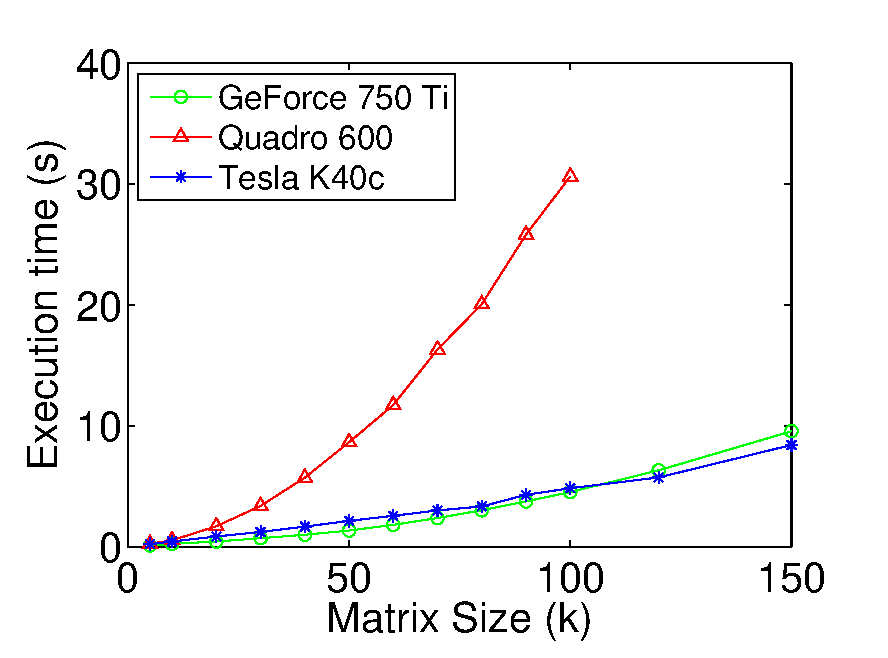
\includegraphics[width=0.3\textwidth,height=1in]{svd_val_gpus}
    \label{fig:svd_val}
  }
  \subfigure[Profiling Data]
  {
    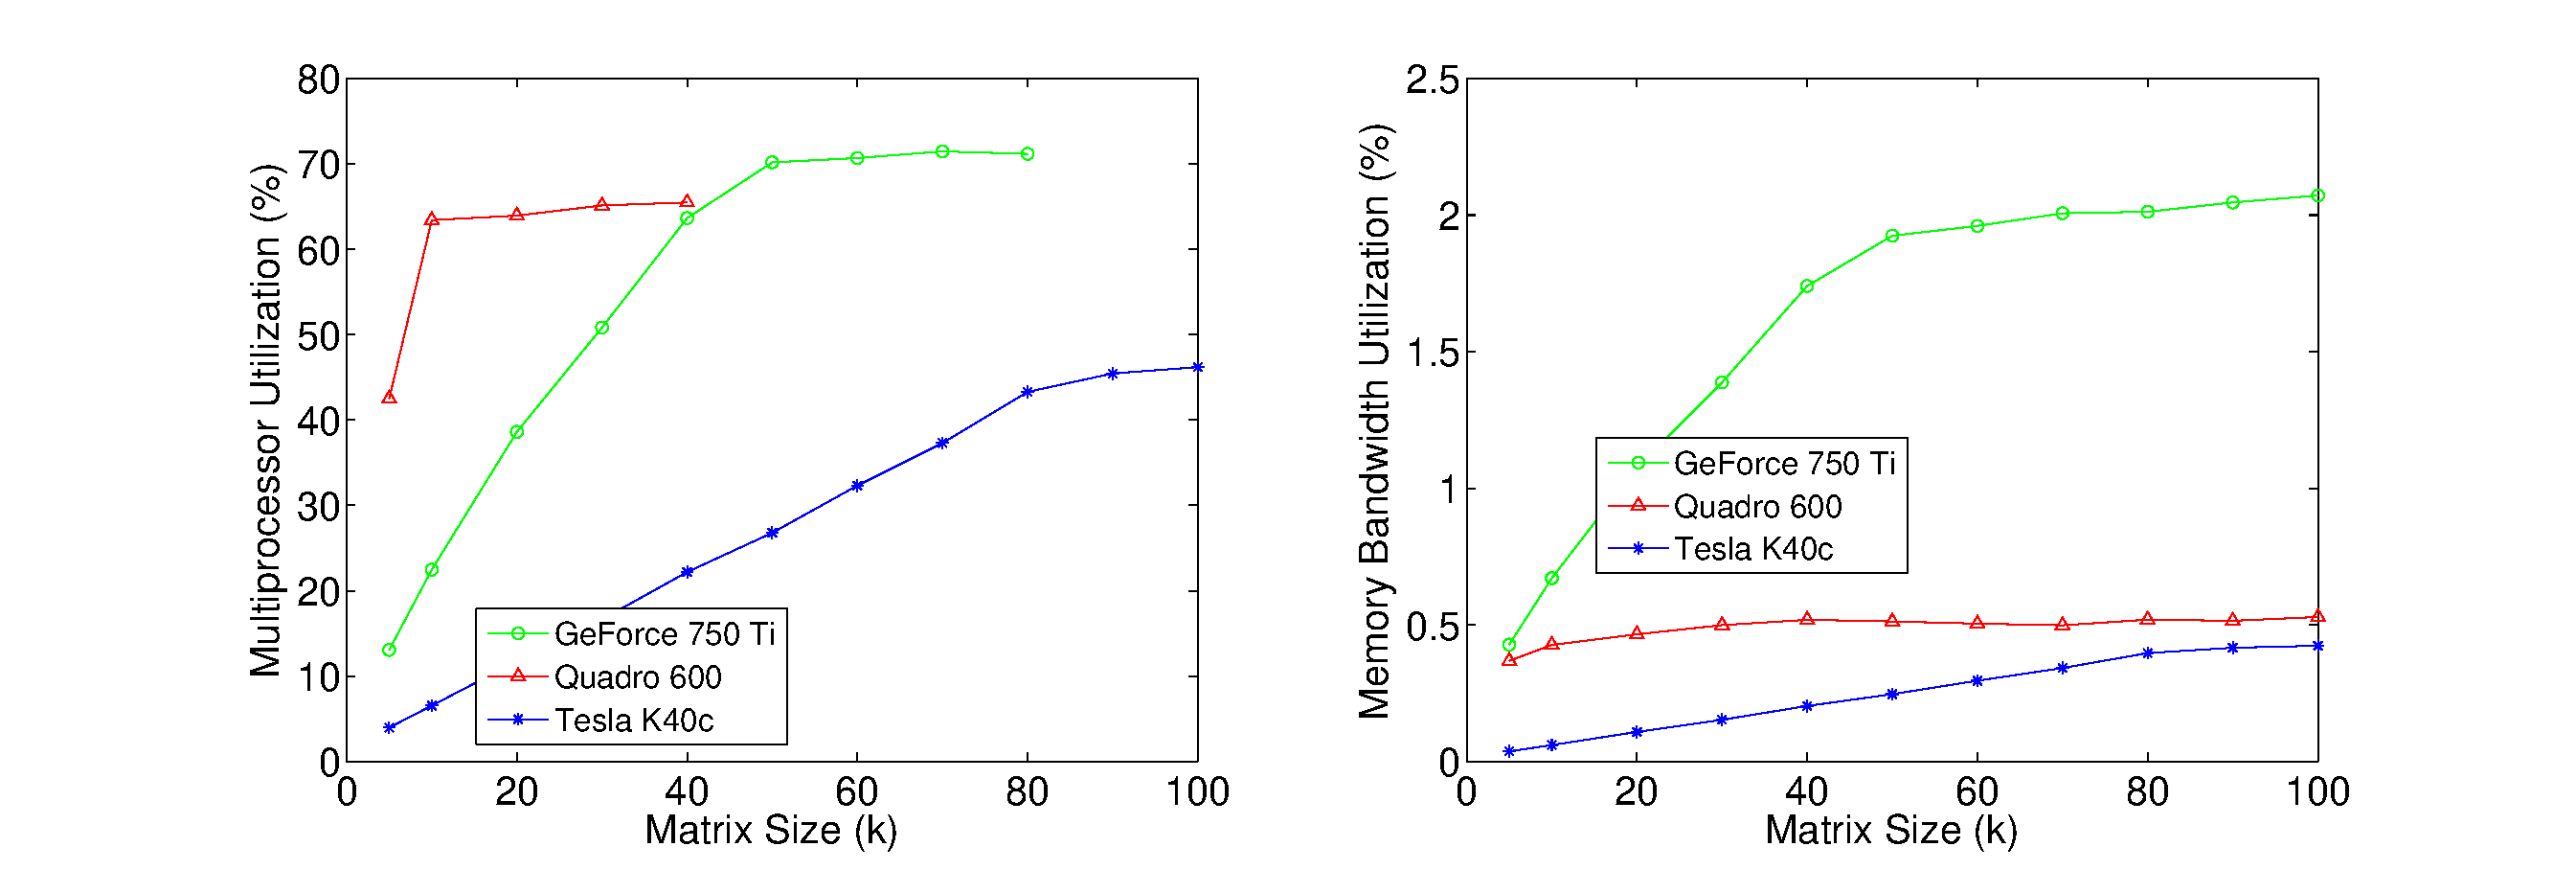
\includegraphics[width=0.6\textwidth,height=1in]{svd_val_gpus_prof}
    \label{fig:svd_val_prof}
  }
\vspace{-0.1in}
  \caption{Singular Value Kernel on Different GPUs}
  \label{fig:svdval}
\vspace{-0.3in}
\end{figure}

Figure \ref{fig:svd_val} shows the execution time of calculating singular values with our ``equal number division'' design on different GPUs with single-precision floating point.
Quadro has the worst performance, while performance of GeForce and Tesla are close to each other.
In particular, When the matrix size is less than $100K$, GeForce is slightly better. Otherwise, Tesla is better. 

To understand the reasons
of such performance differences, we conduct a series of profiling experiments.
Figure \ref{fig:svd_val_prof} shows the thread activity and memory bandwidth utilizations of singular value kernels on different GPUs, for matrices of size up to 
100K (unfortunately we are unable to get profiling data for matrices of larger size due to the overflow of profiling counters). 
The figure shows that the thread utilization reaches 70\% on Quadro and GeForce, and 50\% on Tesla. 
But the memory bandwidth utilization is only 0.1\%-2\%.
The main reason is that singular value computations rely on the fast shared memory
of GPUs due to its low memory requirements. That is, finding the singular
values is rather CPU-bound than memory-bound. 
As a result, the performance is determined largely by the number of CUDA cores and the ratio of thread activity on a GPU.

\subsubsection{Singular Vector Computation}
Figure \ref{fig:svd_vec} shows the execution time of singular vector kernel on different GPUs. 
It is easily seen that GeForce is about 8 times faster than
Quadro. This is because GeForce has a much higher memory bandwidth
than Quadro.
In addition, the device memory read/write transactions of GeForce are only 1/6 and 1/4 of those of Quadro, respectively.
The performance on Tesla is slightly better than that on GeForce.
Tesla has nearly the same device memory read transactions as GeForce does, while 3 times more write transactions than GeForce.
Yet Tesla is still the winner of the three because of its extremely high
bandwidth as listed in Table~\ref{tab:spec}.

\begin{figure}[hbpt]
\vspace{-0.3in}
\centering
  \subfigure[Execution time]
  {
    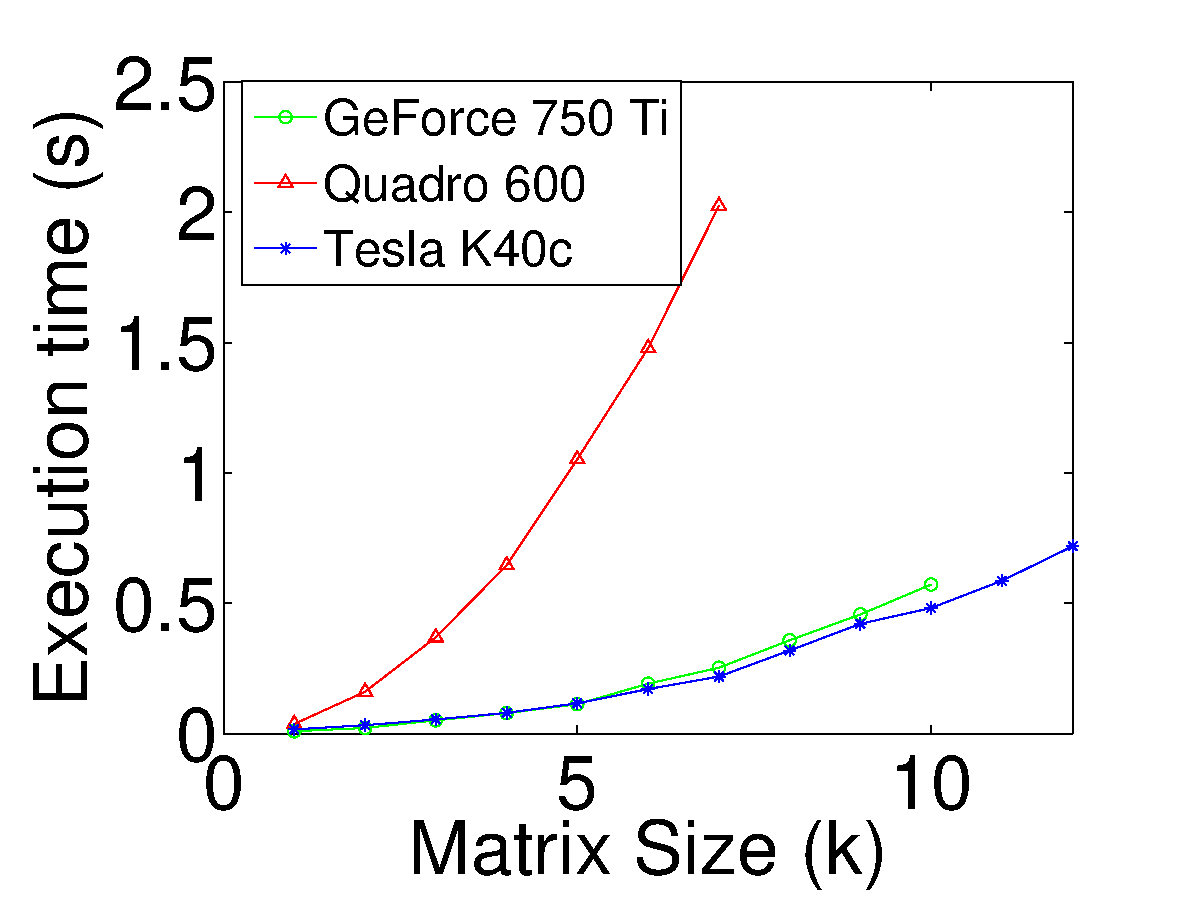
\includegraphics[width=0.3\textwidth,height=1in]{svd_vec_gpus}
    \label{fig:svd_vec}
  }
  \subfigure[Profiling Data]
  {
    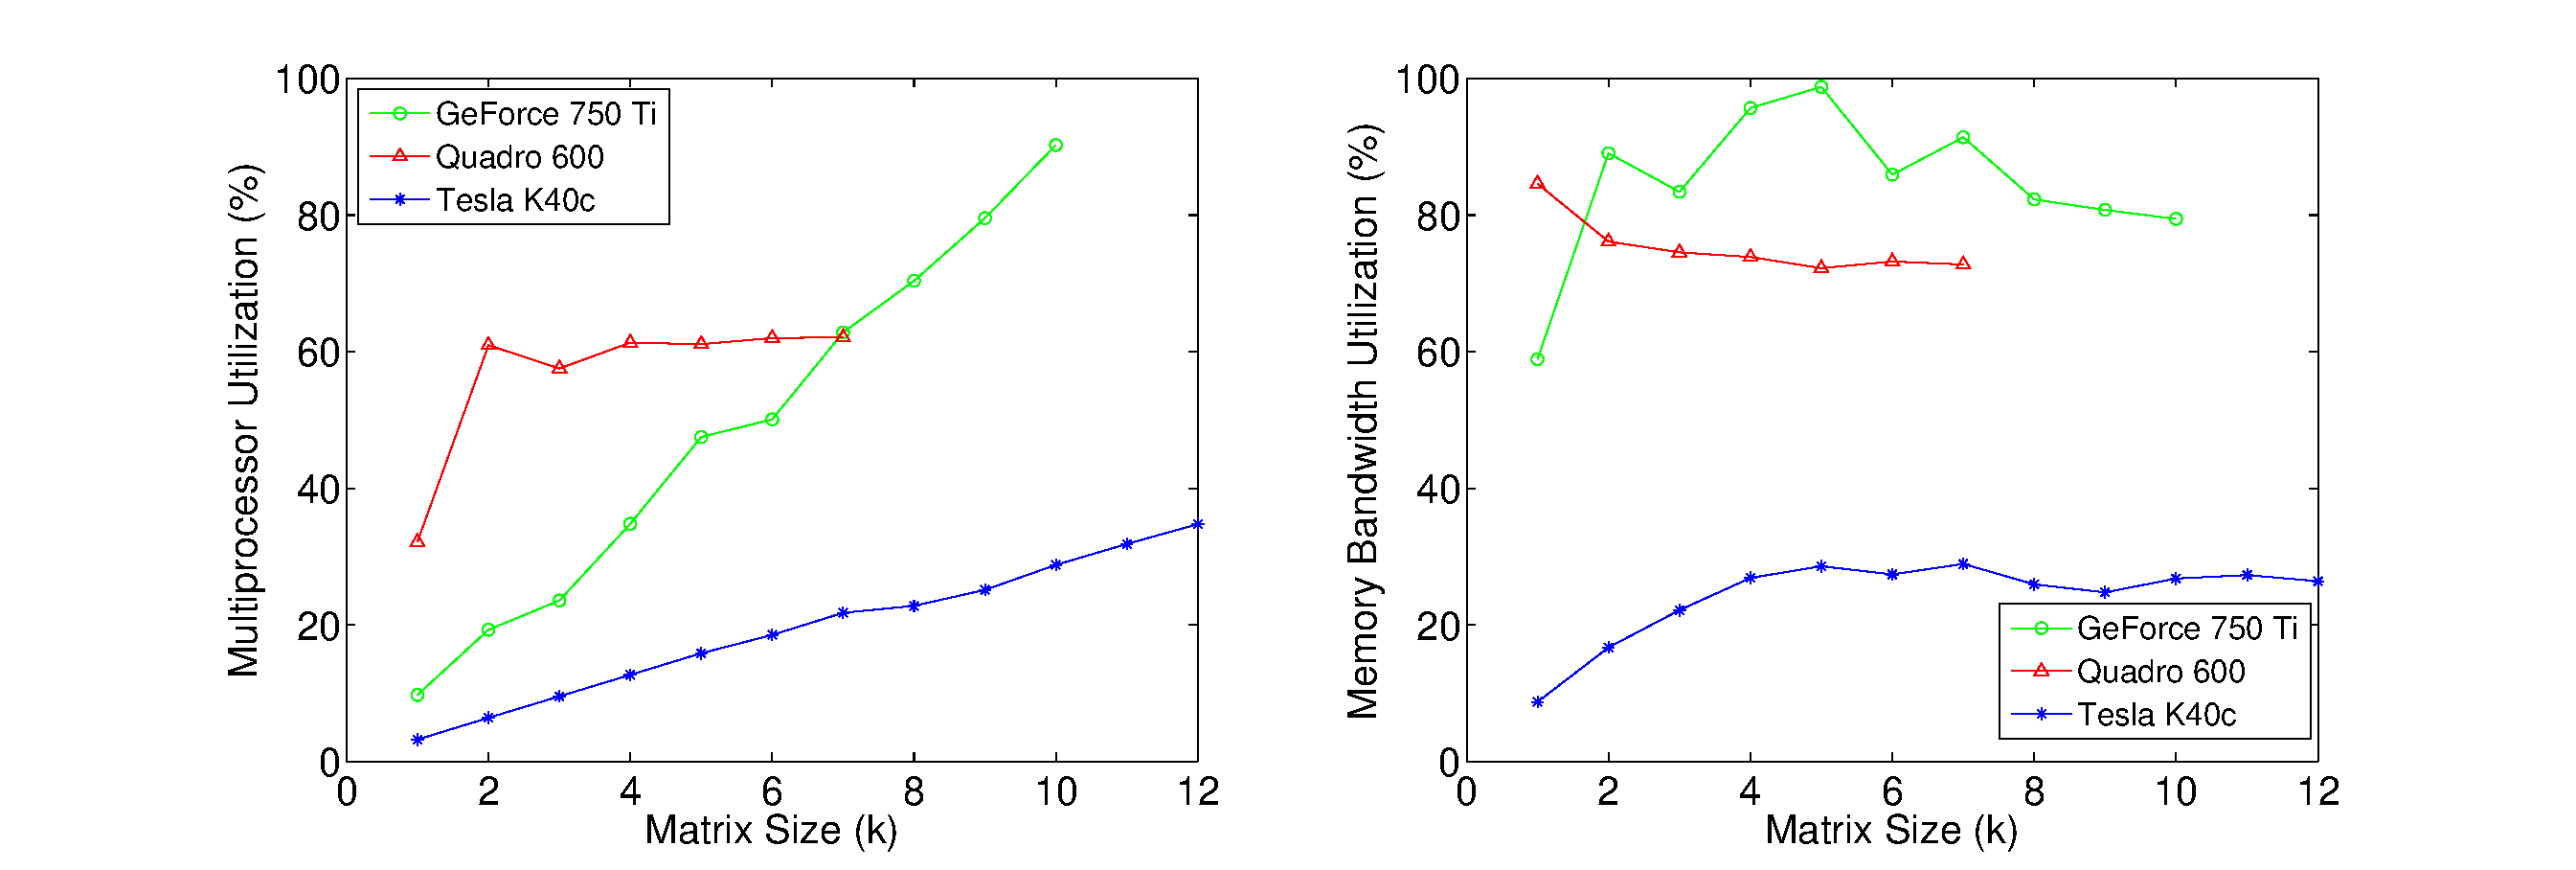
\includegraphics[width=0.6\textwidth,height=1in]{svd_vec_gpus_prof}
    \label{fig:svd_vec_prof}
  }
\vspace{-0.1in}
  \caption{Singular Vector Kernel on Different GPUs}
  \label{fig:svdvec}
\vspace{-0.3in}
\end{figure}

Figure \ref{fig:svd_vec_prof} shows thread and memory bandwidth utilizations of singular vector design on different GPUs. 
We can see from the figure that Quadro and GeForce reach a high memory utilization (80\%-99\%), while the memory utilization of Tesla is around 30\%. 
We also observe that when the matrix size is larger than 2K, the thread utilization keeps stable on Quadro. 
This is because the ratio of stall caused by memory is 70\%, implying that there are a lot of threads waiting on data transfer.


\if 0
\subsection{Performance on a Multi-GPU Platform}

%Scaling the BT algorithm with multiple GPUs is our solution to
%matrices of substantial large sizes such as 1 million on each dimension.
Our solution for matrices of substantially larger sizes such
as 1 million on each dimension is to scale the BT algorithm
with multiple GPUs.
As in our experimental platform, the multiple GPUs in a server may differ
in architecture and performance, thus we need to balance the load on them
to achieve the best speedup.

\subsubsection{Load Balance}
Figure \ref{fig:pthread} shows the total execution times with load distributed to the two GPUs
(Quadro 600 and GeForce 750 Ti) for different matrix sizes on our server.
The x-axis represents the percentage of singular vectors calculated on Quadro 600 (with the rest on GeForce 750 Ti).
The y-axis is the execution time.
%The red cycles highlight the minimum execution time of possible workload distributions.
%The blue curves can be separated into two parts by red points.
%The left ones are dominated by GeForce 750 Ti, while the right ones are contributed by Quadro 600.
%Since Quadro 600 has a worse performance than GeForce 750 Ti, less work is allocated on it.
%We can see that for matrices larger than 3K, a 16\%-84\% partition of the workload
%on Quadro 600 and GeForce 750 Ti yields the best performance. 
A red cycle
highlights the spot where minimum execution time is reached
for each matrix size. We can see that for matrices larger than
3K, a partition of 15\% (Quadro) vs. 85\% (GeForce) yields the
best performance. We believe that this is because 
GeForce has 5 times more effective cores than Quadro.
\begin{figure}[hbpt]
\centering
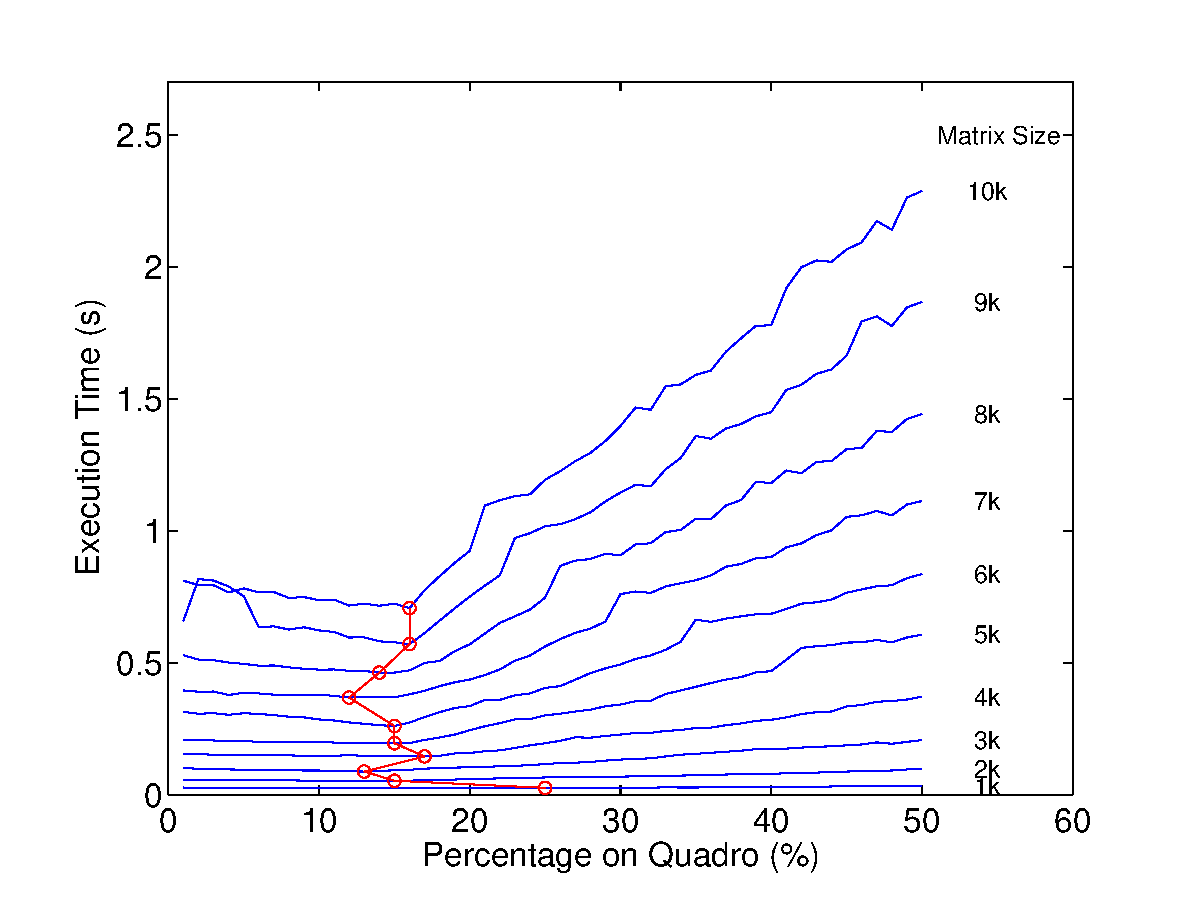
\includegraphics[width=0.38\textwidth]{pthread}
\caption{Load Balance on GeForce and Quadro}
\label{fig:pthread}
\vspace{-0.15in}
\end{figure}
\fi

\subsection{Huge Size Result}
\if 0
Table \ref{tab:hresult} gives the execution times for huge size matrices on a single GeForce, a single Quadra, and both of them with the optimal load balancing as shown in Figure~\ref{fig:pthread}.
When the matrix size is larger than 100K, a single Quadro is not able to calculate the whole SVD.
The GeForce can calculate the whole SVD until the matrix size reaches to 200K.
When the matrix size becomes larger than 200K, our bisection algorithm on GeForce cannot converge due to the accuracy of IEEE single-precision floating point number on GeForce.
When we use double-precision floating numbers on Tesla, our BT implementation works well even when the matrix size reaches one million.
%The GeForce has 4-5X speedup compared to Quadro.
%The right column shows the best execution time and its corresponding workload on two GPUs.
%GeForce is responsible for 80\%-85\% workload, and Quadro taks other part.
%The speedup of 2 GPUs over GeForce is around 1.2.

\begin{table}[h]
\caption{Performance with Very Large Matrix Sizes}
\centering
\begin{tabular}{|c|c|c|c|}
\hline
Matrix Size & GeForce & Quadro & GeForce + Quadro \\ \hline
% 10K*10K    &   0.8s  &  4.6s  &   0.7s (85\%) / 0.7s (15\%) \\ \hline
% 20K*20K    &   2.9s  &   18s  &   2.6s (85\%) / 2.7s (15\%) \\ \hline
% 30K*30K    &   6.7s  &   37s  &   5.9s (85\%) / 5.6s (15\%) \\ \hline
% 40K*40K    &    12s  &   63s  &    10s (85\%) / 9.5s (15\%) \\ \hline
 50K*50K    &    19s  &   96s  &    16s (84\%) /  15s (16\%) \\ \hline
 80K*80K    &    50s  &  238s  &    43s (84\%) /  40s (16\%) \\ \hline
 100K*100K  &    84s  &  393s  &    71s (83\%) /  67s (17\%) \\ \hline
 120K*120K  &   134s  &     -  &   113s (82\%) / 102s (18\%) \\ \hline
 150K*150K  &   245s  &     -  &   203s (81\%) / 194s (19\%) \\ \hline
 180K*180K  &   412s  &     -  &   340s (80\%) / 337s (20\%) \\ \hline
 200K*200K  &   555s  &     -  &   453s (80\%) / 450s (20\%)  \\ \hline
\end{tabular}
\label{tab:hresult}
\vspace{-0.22in}
\end{table}
\fi

Table \ref{tab:hugeResultTesla} shows the performance of huge size matrix with double-precision floating-point numbers on a single Tesla and two Tesla GPUs on a server. For two Telsa GPUs, we compared static workload allocation (50\%/50\%) and dynamic allocation where each GPU is tracked constantly by the host CPU and assigned new workload as soon as it finishes the current kernel. 
%Results that the SVD of a 1 million by 1 million matrix can be calculated with a single Telsa in 54801 %seconds, and with two Telsa GPUs in 35607 seconds, a 1.54 speedup.
When matrix size reaches 1 million by 1
million our BT algorithm reaches the results in 54801 seconds
with a single Telsa, and 35607 seconds with two Telsa GPUs. This is a 1.54X speedup.
\begin{table}[h]
\vspace{-0.3in}
\caption{Performance of Huge Size Matrix with double floating-point on Tesla}
\vspace{-0.1in}
\centering
\begin{tabular}{|c|c|c|c|}
\hline
Matrix Size &  Tesla  & Static & Dynamic \\ \hline
% 10K*10K    &   1.5s  &  1.9s / 1.2s &  0.9s / 2.5s \\ \hline
% 20K*20K    &   7.9s  &  7.4s / 5.7s &  3.1s / 10s \\ \hline
% 30K*30K    &    25s  &   17s /  14s &  12s  / 19s \\ \hline
% 40K*40K    &    38s  &   27s /  24s &  26s / 26s \\ \hline
% 50K*50K    &    71s  &   50s /  45s &  44s / 44s \\ \hline
% 80K*80K    &   180s  &  121s / 103s &  111s / 116s \\ \hline
 100K*100K  &   341s  &  217s / 189s &  210s / 202s \\ \hline
% 120K*120K  &   524s  &  326s / 286s &  311s / 311s \\ \hline
 150K*150K  &   864s  &  524s / 467s &  498s / 507s \\ \hline
% 180K*180K  &   966s  & 1207s / 532s &  602s / 607s \\ \hline
 200K*200K  &  1407s  &  955s / 827s &  849s / 858s \\ \hline
% 250K*250K  &  1949s  & 1286s / 1118s & 1199s / 1204s\\ \hline
 300K*300K  &  3490s  & 2234s / 1906s & 2123s / 2110s\\ \hline
 400K*400K  &  6559s  & 4110s / 3709s & 3853s / 3871s\\ \hline
 500K*500K  & 12282s  & 7371s / 6916s  & 7148s / 7129s\\ \hline
 800K*800K  & 40311s  & 22454s / 21627s &  22046s / 22026s   \\ \hline
 1000K*1000K & 54801s  & 36119s / 35071s   &  35587s / 35607s \\ \hline
\end{tabular}
\label{tab:hugeResultTesla}
\vspace{-0.5in}
\end{table}

\subsection{Profiling Analysis of GPU Kernels}

\subsubsection{Comparison of Two Different Singular Value Designs}
We compare the execution time on two different singular value kernels:
``equal length division'' versus ``equal number division''. Each
method has two phases: (1) divide the interval into subintervals and
(2) calculate singular values in each subinterval.
%For the length division design, we selects the minimal execution time corresponding to red point curve in figure \ref{fig:length_block_num}.
%For the number division design, we selects the minimal number of blocks that is able to allocated, since the execution time does not vary much between the minimal number of blocks and the optimal nubmer of blocks.
\begin{figure}[hbpt]
\centering
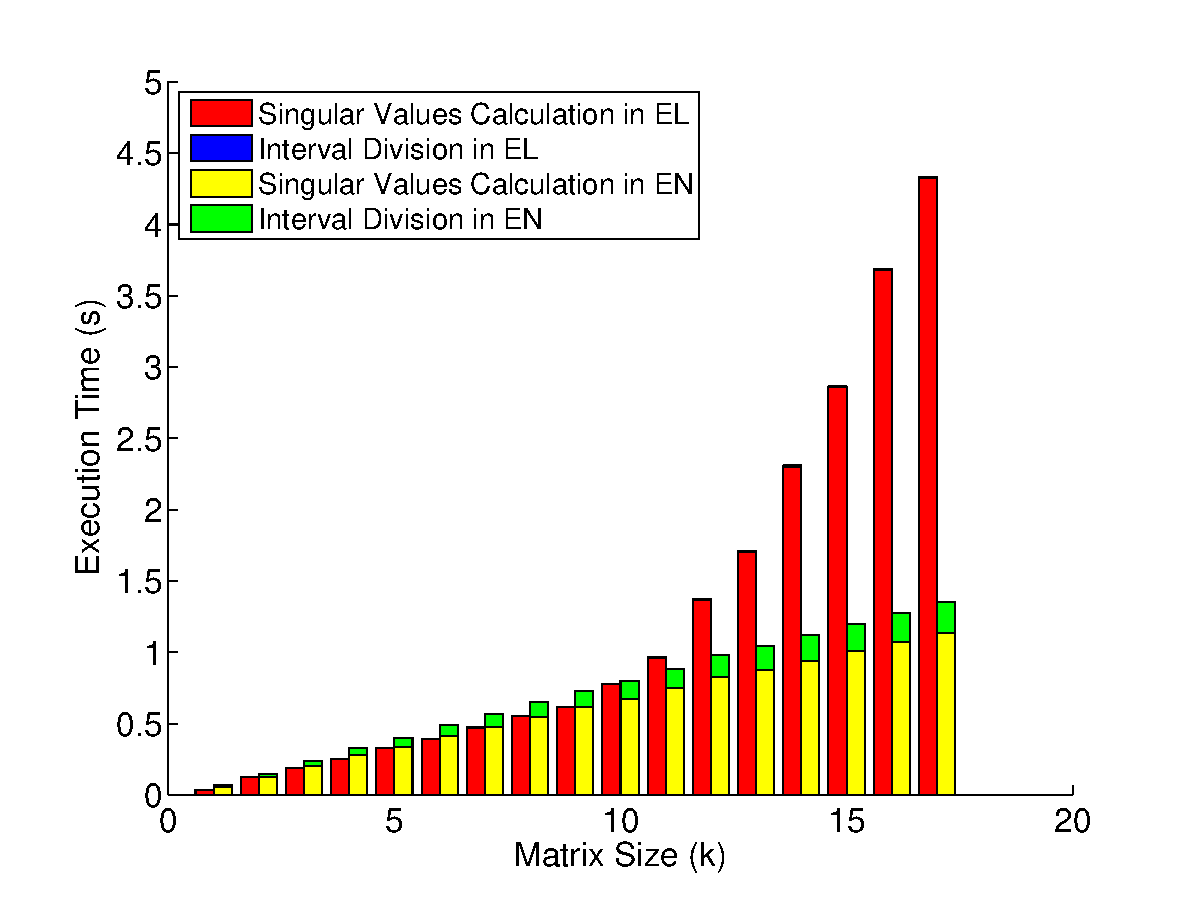
\includegraphics[width=0.4\textwidth]{compare_value_kernel}
\caption{Comparison of Equal Length Division and Equal Number Division. ``Interval Division in EL'' is negligible. }
\label{fig:compare_value_kernel}
\vspace{-0.10in}
\end{figure}
Figure \ref{fig:compare_value_kernel} shows the detailed execution time breakdown for each phase of both methods (``Interval Division'' time for ``equal-length division'' is negligible) on Tesla K40c.
From the figure, we can see that when the matrix size is less than 9K, the equal length division version runs a little faster than equal number division version.
However, when the matrix size exceeds 9K, the execution time of the equal length division version increases dramatically, while the execution time of equal number division version still rises linearly.
And in this case, 
%even the time to divide the interval is noticeably large, the balanced number
%of singular values in a subinterval helps improving the overall performance.
even though the time to divide the interval is noticeably
large, the balanced number of singular values in a subinterval
still yields much better performance.
Thus, the equal number division version is obviously the winner when the matrix size becomes larger than 9K.

\subsubsection{Memory Access Optimization}
We evaluate the memory optimization techniques on improving the performance
of singular vector calculation. As depicted in Figure \ref{fig:transaction},
\begin{figure}[hbpt]
\centering
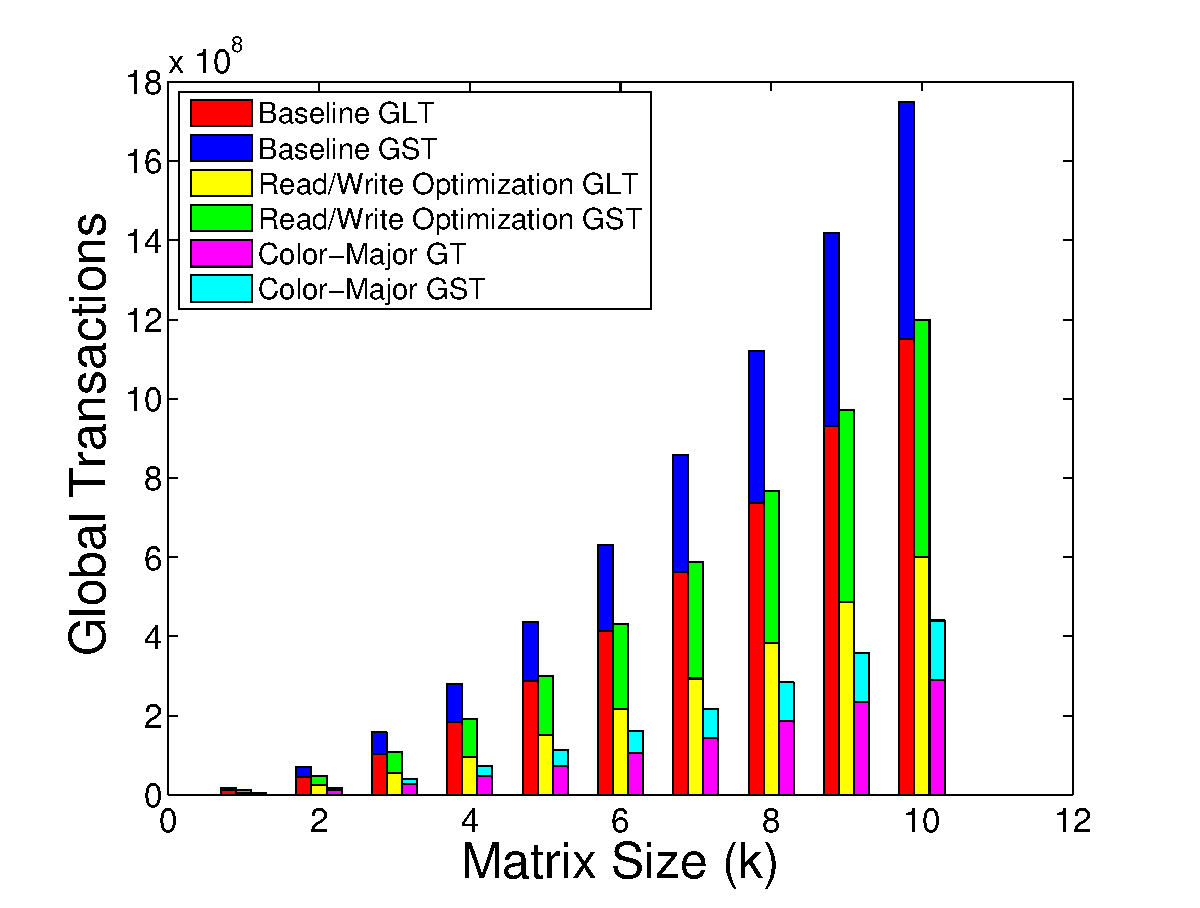
\includegraphics[width=0.4\textwidth]{transaction}
\caption{Memory Transactions on Singular Vector Design}
\label{fig:transaction}
\vspace{-0.15in}
\end{figure}
in the baseline design,
Global memory Load Transactions (GLT) are about twice of the Global memory Store Transactions (GST) on the global memory.
As there are 50\% of global memory transfers are read-after-write, we improve the memory access performance by copying these values into the local memory and shared memory of the GPU. As a result, the GLT are reduced by 50\% compared to the baseline, while the GST remains the same, labeled as ``Read/Write Optimization'' in Figure \ref{fig:transaction}. The speedup on singular vector calculation reaches to 1.2X compared to the baseline.
Changing the matrix arrangement from row-major to column-major in the global memory 
reduces GLT and GST by 50\% and 25\%, respectively, compared to ``Read/Write optimization''. 
This is because column-major matrix have coalesced global memory accesses, which saves hundreds of transactions per thread. The speedup rises up to 4.5X compared to the baseline.

\if 0
\subsubsection{Comparasion of Singular Vector Designs}
Figure \ref{fig:vector_kernels} shows the impact of memory optimizations on singular vector computation.
The column-major matrix with local memory has a better performance than the other versions.
%\begin{figure}[hbpt]
%\centering
%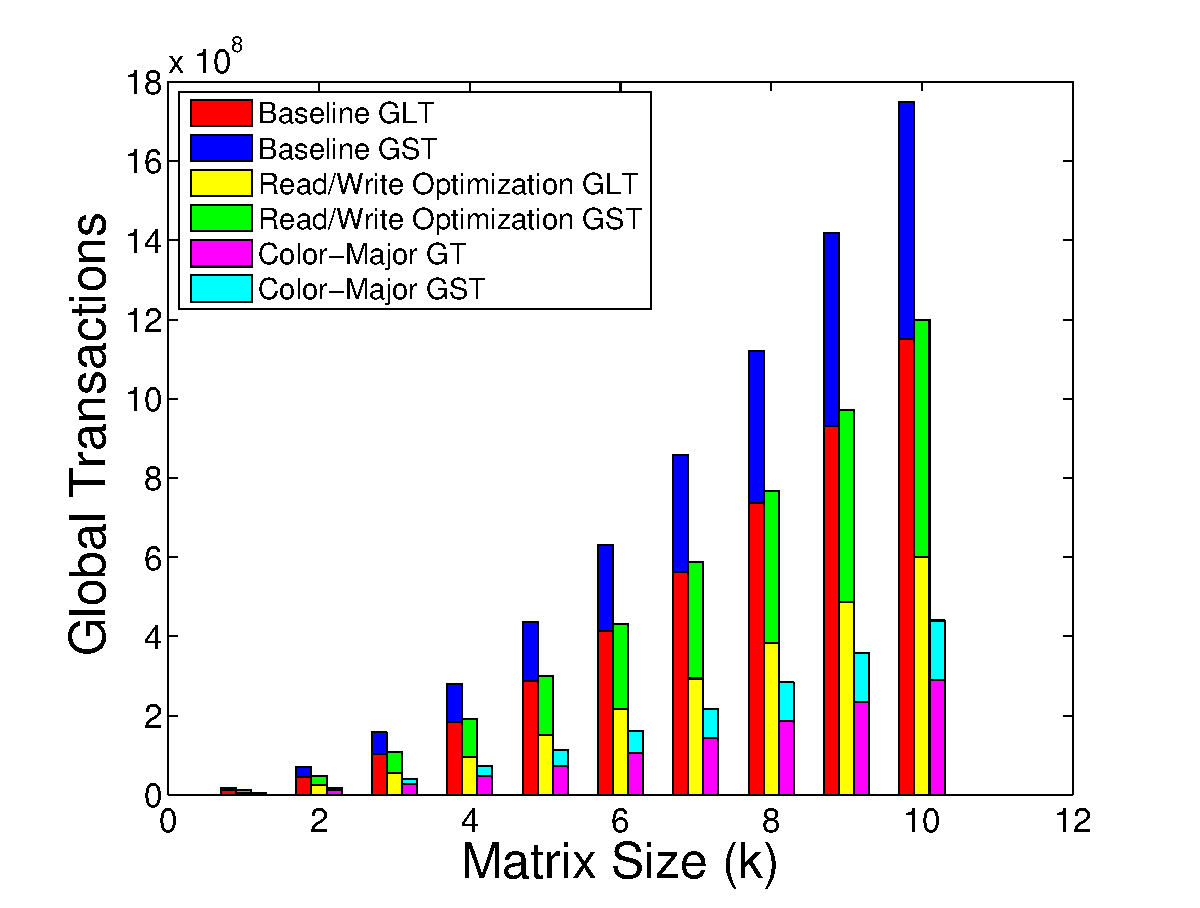
\includegraphics[width=0.5\textwidth]{transaction}
%\caption{Transactions on Singular Vector Design}
%\label{fig:transaction}
%\end{figure}
\begin{figure}[hbpt]
\centering
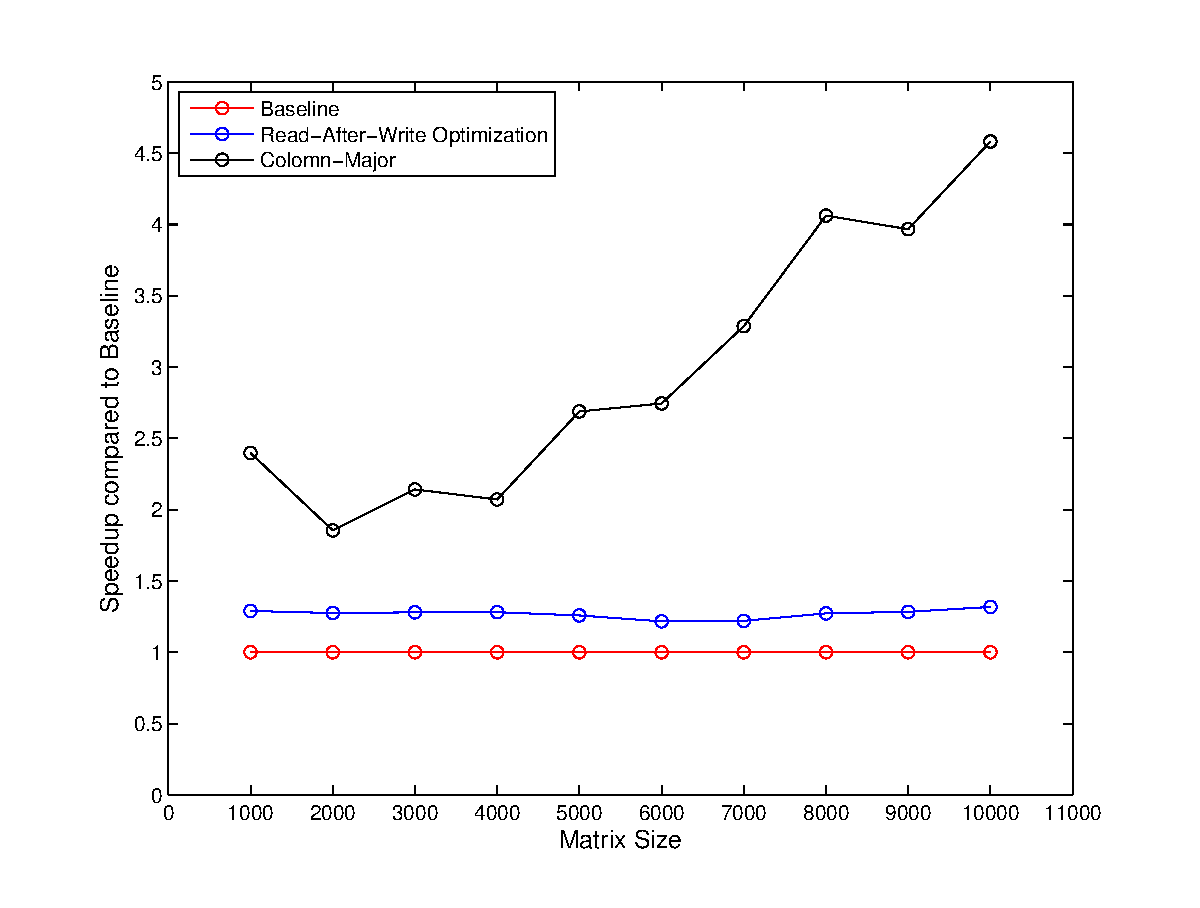
\includegraphics[width=0.5\textwidth]{vector_kernels}
\caption{Performance on Singular Vector Kernels}
\label{fig:vector_kernels}
\end{figure}
\fi

\if 0
\subsubsection{Tolerance in Bisection Algorithm}
Since the bisection algorithm is an approximate algorithm to calculate the singular values, we should test the effect of different error tolerance.
The error tolerance $err$ means that the error between the singular values of our algorithm and the actual singular values are less than $err$.
It determines the accuracy of singular value and therefore the orthogonality of singular vectors.
As we know, the more accuracy of singular values are, the more execution time should be spent.
However, it is important to know the incremental execution time to determine which error tolerance is suitable for different applications.
We test our algorithm on different error tolerance.
The error tolerance is between $10^{-5}$ to $10^{-16}$ with tenfolder decreasing.

%\textbf{I'm still thinking how to draw this figure.}
\begin{figure}[hbpt]
\centering
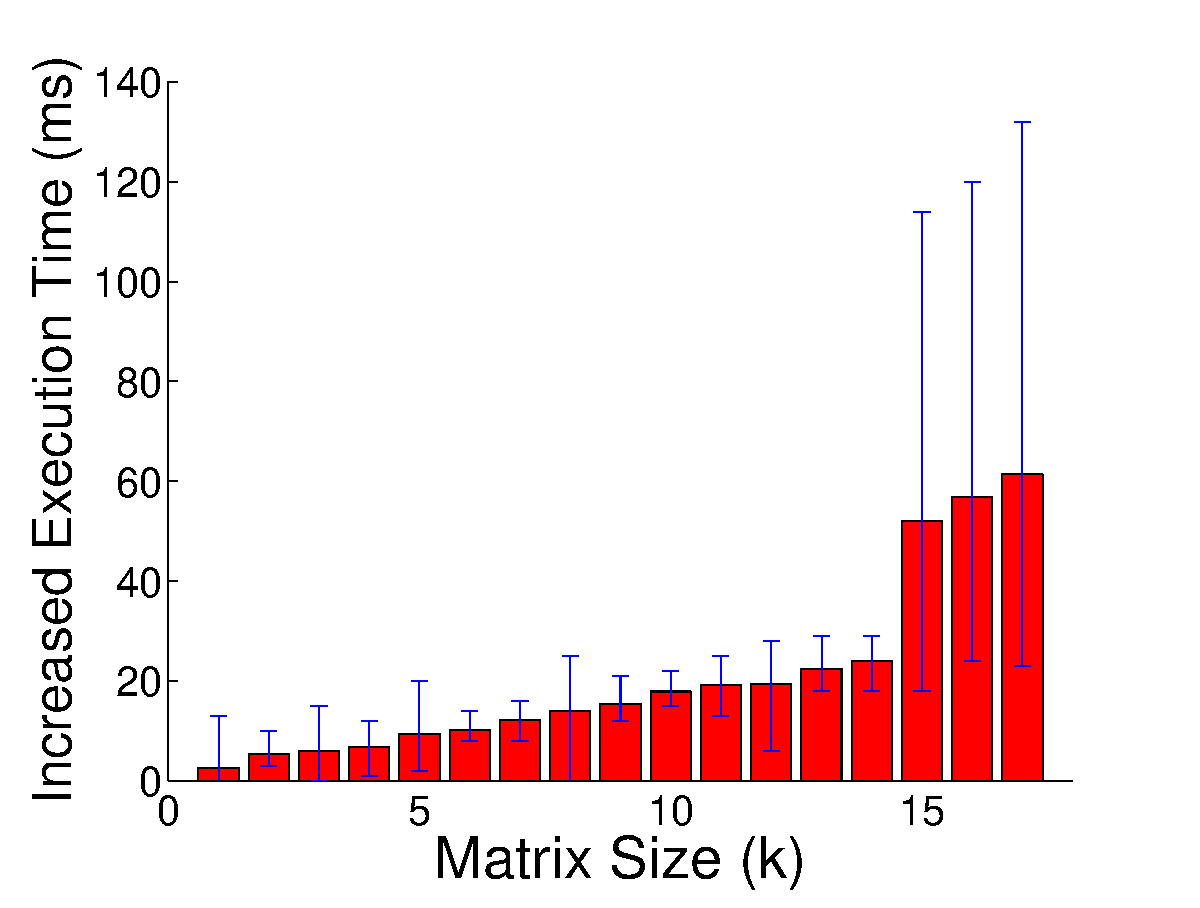
\includegraphics[width=0.5\textwidth]{tolerance}
\caption{Average Extra Execution Time When the accuracy increase Performance Comparision}
\label{fig:tolerance}
\end{figure}
Figure \ref{fig:tolerance} shows the average increased execution time when the accuracy of singular values goes up a higher level on different matrix size.
In other word, it shows the average increased execution time when the error tolerance becomes smaller from $10^{-x}$ to $10^{-(x+1)}$.
From the figure, we can see that when matrix size is smaller than 12000, the additional execution time is only less than $20 ms$ when the error tolerance rises a level.
When the matrix size is larger than 15000, the additional execution time is a little higher about $40 ms$ per level.
\fi


\if 0
\subsubsection{Optimal Block Size}
In our ``equal length division'' design for singular value computation, the size of a block heavily determines the execution time because the most time-consuming block is the critical path. 
We conduct a series of experiments to obtain the optimal block size for different matrices.
%\begin{figure}[hbpt]
%\centering
%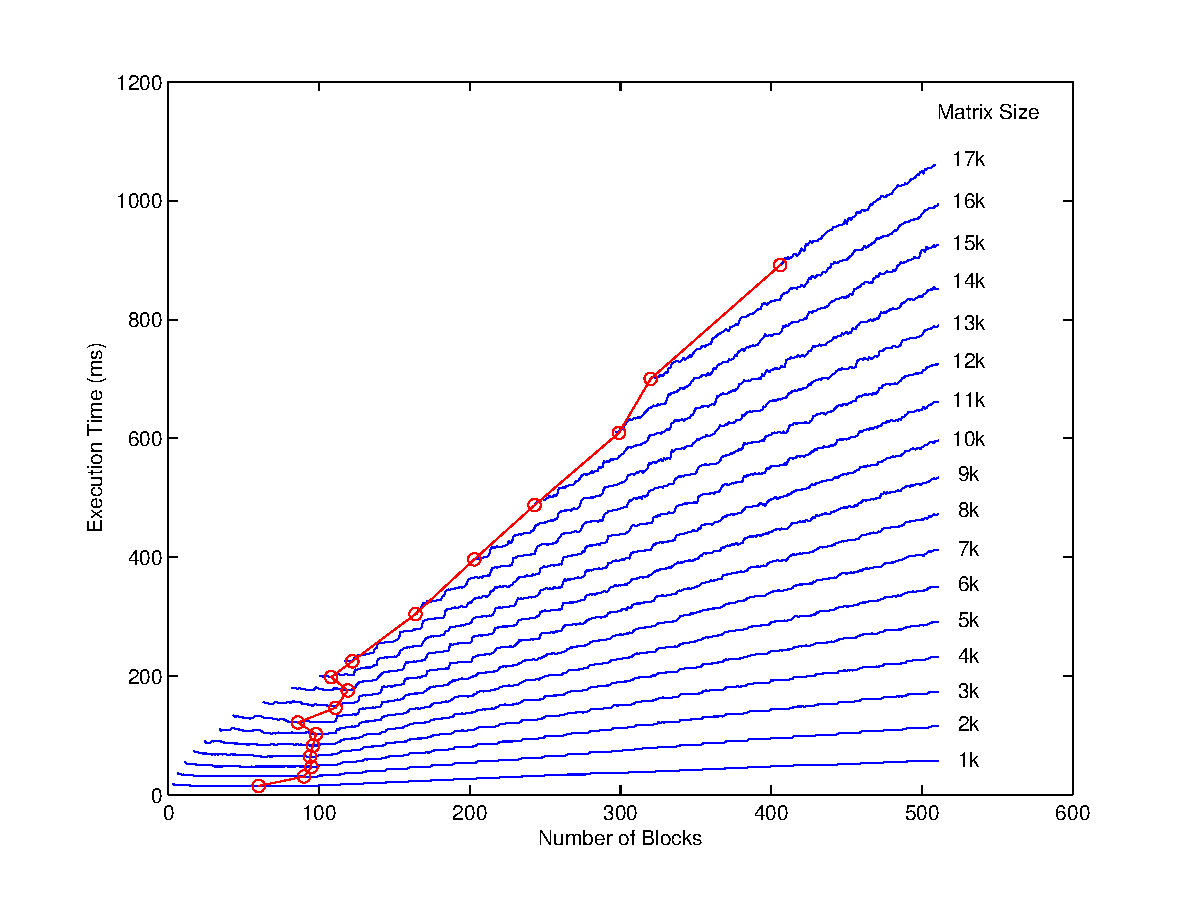
\includegraphics[width=0.5\textwidth]{length_block_single}
%\caption{The optimal block number of different matrix size with single precision on GeForce 750 Ti}
%\label{fig:length_block_single}
%\end{figure}
\begin{figure}[hbpt]
\centering
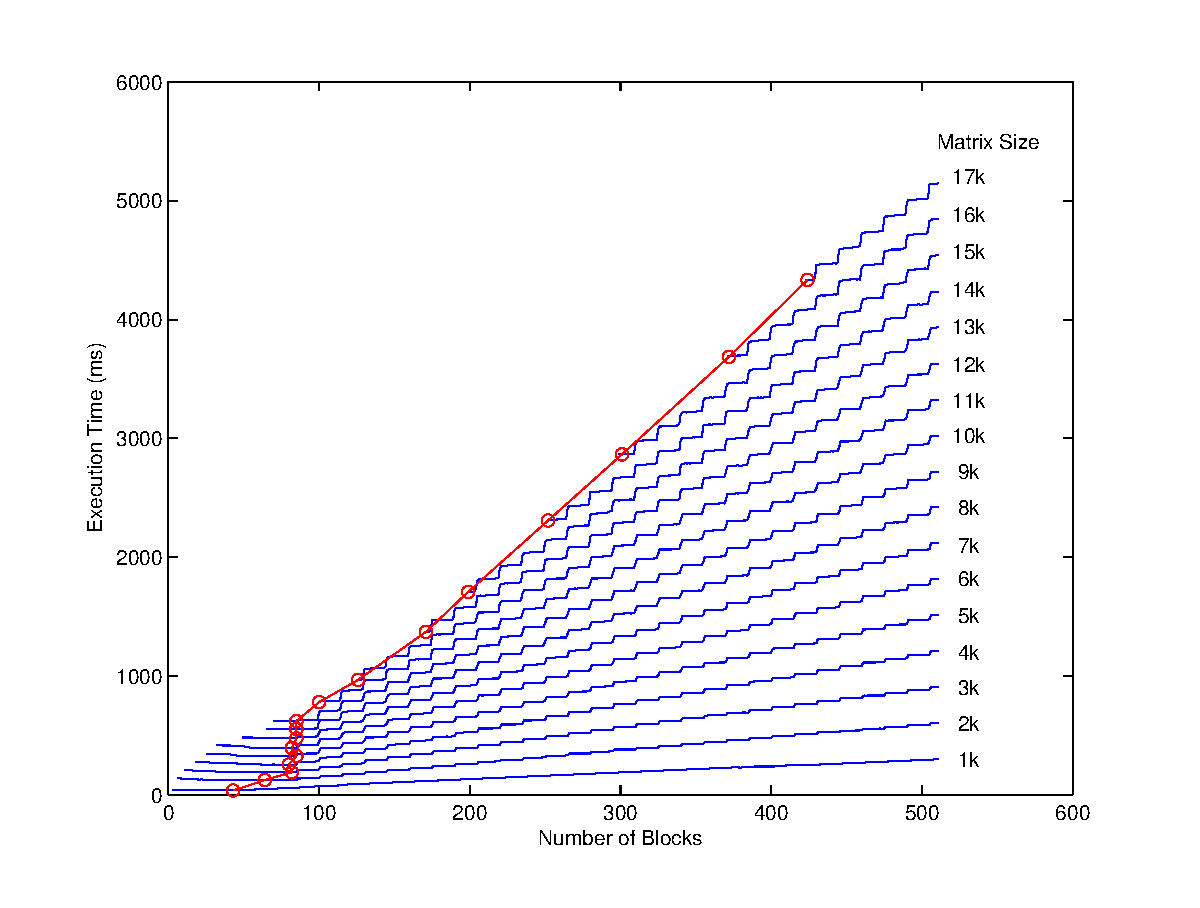
\includegraphics[width=0.5\textwidth]{length_block_num}
\caption{The optimal block number of different matrix size with double precision on Tesla K40c}
\label{fig:length_block_num}
\end{figure}
Figure \ref{fig:length_block_num} shows the execution time of obtaining all the singular values with different number of blocks for a variety of matrix sizes on GPU Tesla K40c with double precision.
The blue wavy curves show the relationship between the execution time and the number of blocks (the matrix size listed on the right side).
From the curves, we can see that the execution time rises when the number of blocks increases.
The left point of the wavy curve shows the minimal number of blocks should be allocated when the matrix size is identified.
In other words, the number of blocks should not be less than the left point on the wavy curves.
When matrix size becomes large, the left point in wave curve trends to a large number of blocks.

The red circle curve in the figure shows the optimal number of blocks with minimal execution time on different size.
we can see that the optimal number of blocks increases when matrix size is less than $3k$,
keeps stable when matrix size is in the range of $3k$ to $9k$,
and becomes the minimal number of blocks when matrix size is lager than $9K$.
Actually, when the block number is close to the optimal number, the execution time does not change too much.
Due to the uncertainty of the input matrix, the optimal block number may vary slightly.
Thus, it is not necessary to select the exact optimal block number.
But it is better to select the number of blocks around the optimal one.

%Figure \ref{fig:length_block_single} is another experimental results on GeForce 750 Ti GPU with single precision.
%The curves are very similar with the curves in Figure \ref{fig:length_block_num}.
%However, the optimal number of blocks shifts right to be a large number because GeForce has a better architecture than Tesla.
%The reason of the optimal number of blocks is determined by the CUDA cores.
%The Tesla K40c has 15 multiprocessors (MP) and 192 CUDA cores per MP.
%Thus, the total CUDA cores are $2880$ in Tesla K40.
%The GPU code is actually executed in groups of 32 threads called a warp concurrently.

%The optimal GPU block size is not the less, the better.
%It depends on the number of singular values in the subintervals.
%If one have more, GPU will have to wait.
%If all subintervals have the number of singular deviate from the integer multiples of a warp. The GPU efficiency will be less.

\fi




\vspace{-0.4in}
\section{Related Work} \label{sec:related}
\vspace{-0.1in}
General purpose GPUs become important processing engines for computationally intensive workloads due to their highly parallel computing architectures.
CUBLAS provides many solutions for low-level linear algebra operations supported by Nvidia \cite{cublas}. 
CULA consists of commercial hybrid GPU accelerated linear algebra routines \cite{cula}.
MAGMA aims to achieve high performance and portability across a wide range of multi-core architectures and hybrid systems respectively\cite{magma}.

%However, it does not provide solutions to complex linear algebra problems, such as QR decomposition, LU decomposition and SVD.
%CULA consists of commercial hybrid GPU accelerated linear algebra routines\cite{cula} that support high-level linear algebra operations.
%Among them, the singular value decomposition employs QR algorithm, which is not an effective algorithm when the matrix size becomes significantly large.
%MAGMA aims to achieve high performance and portability across a wide range of multi-core architectures and hybrid systems respectively\cite{magma}.

The first SVD algorithm with CUDA programming is implemented by Sheetal et al.\cite{09IPDPSQR}. With parallelized QR iteration algorithm using CUBLAS library on GPU, they achieved a speedup of up to 8 over the Intel MKL QR implementation.
Liu et al. use a divide-and-conquer approach to solve SVD on a heterogeneous CPU-GPU system \cite{13CFDC}.
It is almost 7 times faster than CULA QR algorithm executing on the same device M2070, and up to 33 times faster than LAPACK.
Vedran\cite{14arxivjacobi} presents a hierarchically blocked one-sided Jacobi algorithm for the singular value decomposition on both single and multiple GPU architectures. 

Drineas et al. \cite{99clustering} provide a clustered SVD algorithm for large matrices. The algorithm divides a set of $n$ points into $k$ clusters, where $k$ is much less than $n$ on CPU.
It is an approximation algorithm to obtain only one subset of singular values
and vectors. Our BT algorithm can compute the complete SVD, thus is not
directly compared with \cite{99clustering}. 



\section{Conclusion}
\label{sec:conclusion}
We present a novel algorithm for computing singular values and vectors called bisection and twisted (BT) algorithm, 
which is implemented on both single GPUs and a multi-GPU platform.
The experimental results show that BT outperforms a number of existing
work on SVD acceleration. %Additionally, BT's scalability is excellent:
One of the major advantages for BT algorithm is its scalability:
we are the first to perform SVD on a matrix of 1 million by 1 million,
using only two GPUs. In the near future, we plan to extend our multi-GPU version of BT
with network middleware such as MPI so that BT algorithm can be further 
extended to distributed GPUs.
%scaled with GPU clusters.


\section*{Acknowledgment}
This work is support in part by the National Science Foundation under grant number ACI-1440737. 

\bibliographystyle{splncs}
\bibliography{ref}

\end{document}
